\documentclass[11pt]{report}

\usepackage[english]{babel}
\usepackage[utf8x]{inputenc}
\usepackage{amsmath}
\usepackage{graphicx}
\usepackage{caption}
\usepackage{subcaption}
\usepackage{float}
\usepackage[left=1.5in, right=1in, top=1in, bottom=1in, includefoot, headheight=13.6pt]{geometry} % margins as suggested in http://codeinthehole.com/writing/writing-a-thesis-in-latex/ 
\usepackage{indentfirst}
\usepackage[colorinlistoftodos]{todonotes}
\usepackage{titlesec}
\usepackage[nottoc,notlot,notlof]{tocbibind}
\usepackage{nth} % allows days formatting. i.e. 1st, 2nd , ..., i-th
\usepackage{url}
\usepackage[toc,page]{appendix}
\usepackage{setspace}

\usepackage{hyperref}
\hypersetup{
    colorlinks,
    citecolor=black,
    filecolor=black,
    linkcolor=black,
    urlcolor=black
}
 
\graphicspath{{images/}}

\titleformat{\chapter}[display]{\normalfont\huge\bfseries}{}{0pt}{\Huge}
\titlespacing*{\chapter}{0pt}{10pt}{40pt}

\renewcommand{\baselinestretch}{1.5}

\newcommand{\HRule}{\rule{\linewidth}{0.5mm}}

% Allow C# Code to be embedded
\usepackage{listings}
\usepackage{xcolor}
\renewcommand{\lstlistingname}{Code}

\lstdefinestyle{sharpc}
{language=[Sharp]C, 
frame=single, 
rulecolor=\color{blue!80!black}, 
keywordstyle=\color{blue}, 
numbers=left,
breaklines=true,
basicstyle=\footnotesize\singlespacing}

\lstdefinestyle{sharpc1}
{language=[Sharp]C, 
frame=single, 
rulecolor=\color{blue!80!black}, 
keywordstyle=\color{blue}, 
numbers=none,
breaklines=true,
basicstyle=\footnotesize\singlespacing}


\begin{document}


\begin{titlepage}
\begin{center}

% Upper part of the page. The '~' is needed because \\
% only works if a paragraph has started.

% Title
\HRule \\[0.4cm]
{ \huge \bfseries A Haptic Device for Graph and Text exploration by People with Visual Disabilities }
\HRule \\[0.4cm]


\includegraphics[width=0.5\textwidth]{../images/St_Andrews_Logo.jpg} %~\\[1cm]

% Author and supervisor
\begin{minipage}{0.4\textwidth}
\begin{flushleft} \large
\emph{Author:}\\
Simone Ivan \textsc{Conte}
\end{flushleft}
\end{minipage}
\begin{minipage}{0.4\textwidth}
\begin{flushright} \large
\emph{Supervisor:} \\
Dr.~Miguel A. \textsc{Nacenta}
\end{flushright}
\end{minipage}

\vfill

% Bottom of the page
{\large \today}

\end{center}
\end{titlepage}
\clearpage\mbox{}\clearpage
\newpage
\section{Abstract}
53/250 WORDS

The use of technology for the blind and the visually impaired is not obvious. Overcoming this digital divide gap is one of today's challenged. In this report I present the Multi-Haptic Tabletop Puck, a tactile feedback input device for touch displays, together with an easy-to-use API and a new sets of dynamic behaviours. \todo[noline]{Improve}
\clearpage\mbox{}\clearpage
\newpage
\section{Declaration}
I declare that the material submitted for assessment is my own work except where credit is explicitly
given to others by citation or acknowledgement. This work was performed during the current academic
year except where otherwise stated.

The main text of this project report is XX,XXX words long, including project specication and plan.

In submitting this project report to the University of St Andrews, I give permission for it to be made
available for use in accordance with the regulations of the University Library. I also give permission for
the title and abstract to be published and for copies of the report to be made and supplied at cost to
any bona de library or research worker, and to be made available on the World Wide Web. I retain the
copyright in this work.
\newpage
\clearpage\mbox{}\clearpage
\newpage
\section{Acknowledgments}
I would like to thank:
\begin{itemize}
\item Miguel A. Nacenta
\item Saad Attieh and Regis
\item The School of Computer Science and the SACHI research group
\end{itemize}
\clearpage\mbox{}\clearpage
\newpage

\tableofcontents{hyperref}{links}
\newpage

\listoffigures
\newpage

\chapter*{Introduction}
\addcontentsline{toc}{chapter}{Introduction}

Technology, in the last decade, has become ubiquitous. Etc..

\begin{enumerate}
    	\item Address what the problem is
        \item Current devices for visually impaired are expensive (examples)
        \item Explain that different approaches have been considered. One of this is the HTP
        \item Explain the vision of the MHTP
  	\end{enumerate}
    
\section*{Haptic feedback technology}
\addcontentsline{toc}{section}{Haptic feedback technology}

    
\section*{Aim}
\addcontentsline{toc}{section}{Aim}

\section*{Project Success}
\addcontentsline{toc}{section}{Project Success}
\newpage
\chapter{Objectives}


\begin{enumerate}
	\item Primary
    \begin{enumerate}
    	\item Design and implement an haptic device for graph exploration by people with visual disabilities.
        \item Design and implement an haptic device for text exploration by people with visual disabilities.
        \item Develop an API to control one or more haptic devices.
        \item Develop an API to easily develop WPF client applications.
        \item Design and implement a new set of dynamic behaviours.
        \item Design and implement a basic application for Graphs exploration.
    \end{enumerate}
    \item Secondary
    \begin{enumerate}
        \item Increase the haptic device resolution.
        \item Allow the haptic device to provide audio-feedback as well.
        \item Design and implement an application for simple mathematical functions exploration.
    \end{enumerate}
    \item Tertiary
    \begin{enumerate}
    	\item Enable the haptic device to be used collaboratively.
        \item Enable the haptic device to sense textures.
    \end{enumerate}
\end{enumerate}

All the primary and secondary objectives have been achieved.\par
The secondary objectives, in semester one, included also the implementation of dynamic pointing. This feature, however, was removed for reasons discussed later in Evaluation chapter \todo[noline]{remember to discuss this}.

In addition to the objectives above, I pursued this project with the following other goals in mind:
\begin{itemize}
	\item Investigate and evaluate the current state of the art.
    \item Develop a device which fits within the current state of the art.
    \item Develop a modular device which can be easily adapted to various conditions and needs.
\end{itemize}
\newpage
\chapter*{Background}
\addcontentsline{toc}{chapter}{Background}

This section addresses various haptic feedback techonologies. One of the main aims of this project is not only to create the next HTP, but also to address some of the limitations of other recent haptic technology. 

Research in haptic visualization has grown significantly in the last 25 years \cite{roberts2007we}. Being able to cover most of the work in haptics is not feasible. I will start by presenting the PHANTOM, one of the most significant haptic devices of the 90s, and then present some more recent work to understand what the current state of the art is and where it is heading. 

\section*{PHANTOM}
\addcontentsline{toc}{section}{PHANTOM}

\begin{enumerate}
	\item User study from Glasgow University on Cartesian Graphs perception
\end{enumerate}
  
\section*{AIREAL}
\addcontentsline{toc}{section}{AIREAL}

Another technology recently developed by Disney Research is AIREAL. AIREAL is (TODO - Describe). 

The main advantages of AIREAL are that it's scalable, inexpensive and can be easily used in public spaces. On the other hand, however, high-resolution tactile feedback represents a major challenge. 

The work presented by Sodhi et Al. seems to be very portable for gaming applications, where "feeling" the environment can enhance a better user experience. Nonetheless, this technology does not seeem particularly suitable for graph exploration, especially for the visually impaired. Text exploration is also not feasible, since AIREAL functions as an output device only, therefore the user cannot query the user for the wanted information.

\section*{Revel}
\addcontentsline{toc}{section}{Revel}

Predecessor is TeslaTouch - revel works the opposite direction

Introducing the concept of ARTactile displays: 
\begin{enumerate}
	\item Extrinsic haptic: integrated in the environment
    \item Intrinsic haptic: augment the user
\end{enumerate}


\section*{FingerFlux}
\addcontentsline{toc}{section}{FingerFlux}

\section*{Changeable Physical Buttons}
\addcontentsline{toc}{section}{Changeable Physical Buttons}

Major problem: display is static. Must be created in advance.

\section*{inFORM}
\addcontentsline{toc}{section}{inFORM}

The Tangible Media Group, MIT, has recently presented inFORM at UIST13. 

(see: \cite{follmer2013inform})

\section*{Conclusion/Summary}
\addcontentsline{toc}{section}{Conclusion/Summary}

\newpage
\chapter{Research and Methodology}

The nature of this project is more research than engineering oriented. It follows that common software development practices, such as SCRUM, were not used. Instead, the development process was articulated in three main phases: background research, hardware and software investigation, and hardware and software development. Each of these phases will be discussed below. 

\section{Project phases}
The background research phase was necessary to understand what the current state of the technology in haptic devices is. This phase was run mainly in the first two months of the project. 

The hardware and software investigation phase consisted in getting familiar with the 3D Printer, the Phidgets API and exploring what possible hardware could be used. For instance, hardware experimentation on Quantum Tunnelling Composite (QTC) was pursued to get pressure input from the device. The final evaluation was negative due to the reduced size of QTC tiles, which do not allow an easy installation on the MHTP. I then decided to use basic a Force-Sensing resistor instead. 

The hardware and software development phase followed the investigation phase logically, but not necessarily temporarily. Both the hardware and the software presented in this report are the product of an iterative exploratory design process. Weekly meetings with the supervisor were arranged. Each meeting consisted in reporting the work done in the previous week, planning the work for the week after and discussing design problems and features. These brainstorming meetings were fundamental in order to achieve the final HaptiQ.

Monthly meetings with Saad Attieh were arranged to discuss various design choices and get direct feedback from a blind person, which I found invaluable. 
One of the aims of this project is develop an haptic device easy to build with an easy-to-use API. An instruction manual on assembling the device is provided \todo[noline]{TODO - Manual}. On the software side, the API has been designed having in mind that the code will be used for future work. Therefore, I wrote extensive XML documentation for the API calls and provided abstract instances, where necessary, to allow future users to extend the API. 

\section{Management software}
Version control systems have been used to facilitate the software development of the API and maintain the 3D Models of the HaptiQ always up-to-date. The Mercurial version control system, managed by the School of Computer Science, has been used from the beginning of the project until almost the very end. On the \nth{18} March 2014, with Régis Ongaro-Carcy joining the project, I decided to switch to GitHub. The main reasons behind this choice are that Régis does not have access to Mercurial repositories within the School of Computer Science and GitHub provides an issue tracking system that facilitates project work with more than one person.  

At the start of the project I used the issue tracker Bugify \cite{bugify}. However, later in the project development process I stopped using this tool because the project evolved too quickly and Bugify slowed down my process rather than speeding it up. 

\section{Testing}
One of the most challenging parts of this project was testing. Being the implemented API highly dependent on both the HaptiQ device and the input device (table, camera, et cetera) the amount of Unit testing was minimal. This required me to manually ran the API multiple times and under various conditions in order to ensure that the software worked properly. A similar approach was undertaken to test the hardware. I regularly checked every part of the hardware to ensure that nothing was broken and that all pieces were installed correctly.
\newpage
\chapter{Ethical Considerations}

No user study was pursued, therefore this project does not have any Ethical Considerations and does not require ethics approval.\newline \par

\section{Collaborations}
This project involved collaborations with two students: Saad Attieh and Rejis Ongaro-Carcy.  

Saad Attieh, University of St Andrews, joined the project as a collaborator, under the approval of the School of Computer Science of the University of St Andrews, in November 2013. Meetings with Saad were established about every month and he has provided very useful feedback on the device design and tactons. 

Régis Ongaro-Carcy, Université de Strasbourg - ISIS, joined the project on the \nth{18} March 2014. Régis is using the HaptiQ as part of his Master's thesis focused on designing a strategic game, based on geographical information, for visually impaired people. He has provided some insightful feedback. While using the API, Régis found some bugs or features that should be added. He reported these issues through the issue tracking system of GitHub.
\newpage
\chapter{Design}

The HaptiQ aims to solve some of the problems identified in the related work. The hardware was developed using an iterative exploratory process. Therefore the design phases largely overlap with the implementation ones. The API provided has also undergone through many iterations. In this chapter I will first discuss the earliest prototypes. Then the 4-HaptiQ and the 8-HaptiQ hardware designs are illustrated. Finally, a detailed overview of the API is provided.

\section{The Hardware}
\subsection{Early Prototypes}
The hardware design of the HaptiQ has been initially based on the HTP design. Similarly to the HTP, the HaptiQ also uses mini-servos to control its actuators. However, while the HTP controls only one actuator, the HaptiQ controls four or eight of them. It immediately follows that as the number of actuators increases, so do the number of servos and the size of the device. In order to minimise the size I designed three main prototypes by sketches (see Figure ~\ref{fig:HaptiQ-early-prototypes}). 

The first prototype extends the rotational axis in the xy plane (see Figure ~\ref{fig:first prototype}). The extension is designed as a gear that allows to choose combinations of three aligned actuators. An additional actuator would then be used to raise the selected actuators. This design reduces the number of servos, but all raised actuators will have the same height. Note that the focus of this design sketch was to minimise the number of servos, that is why actuators are shown as points, similar to Braille displays.

\begin{figure}
        \centering
        \begin{subfigure}[H]{0.5\textwidth}
                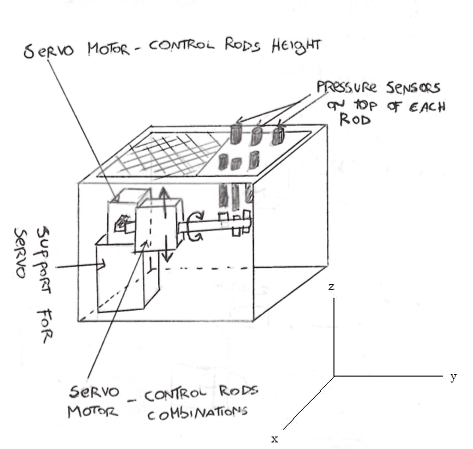
\includegraphics[width=\textwidth,height=\textwidth]{prototype1.png}
                \caption{Grid based}
                \label{fig:first prototype}
        \end{subfigure}%
        ~ %add desired spacing between images, e. g. ~, \quad, \qquad etc.
          %(or a blank line to force the subfigure onto a new line)
        \begin{subfigure}[H]{0.5\textwidth}
                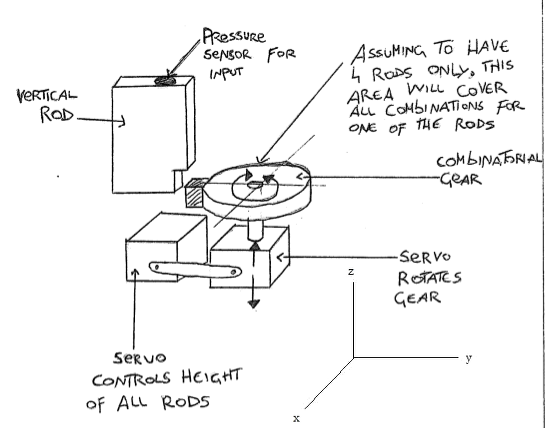
\includegraphics[width=\textwidth,height=\textwidth]{prototype2.png}
                \caption{Gear based}
                \label{fig:second prototype}
        \end{subfigure}
        ~ %add desired spacing between images, e. g. ~, \quad, \qquad etc.
          %(or a blank line to force the subfigure onto a new line)
        \begin{subfigure}[H]{0.5\textwidth}
                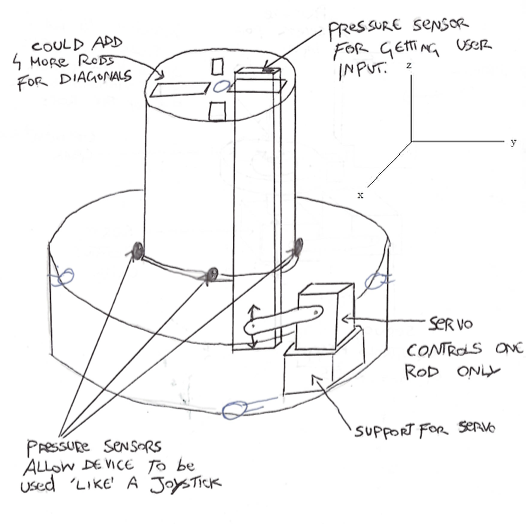
\includegraphics[width=\textwidth,height=\textwidth]{prototype3.png}
                \caption{One servo per actuator}
                \label{fig:third prototype}
        \end{subfigure}
        \caption{HaptiQ early prototypes}\label{fig:HaptiQ-early-prototypes}
\end{figure}

In the second prototype I tried to minimize the total number of servos to two. One servo would be used to rotate a combinatorial gear about the z-axis(see Figure ~\ref{fig:second prototype}). A second servo can then be used to raise the first servo with the gear it controls and all the rods. This approach can be considered very versatile and could allow an high number of actuators by keeping the number of servos always to two. Nonetheless, the actuators would all be at the same heights when raised as in the first prototype. Since height can be used to convey additional information, this prototype was discarded and a third prototype was created.

The third prototype does not focus on minimising the number of servos any more, but rather on the possible functions that could be added to the HaptiQ. In this design each servo controls an actuator only and these are disposed circularly around the centre of the device (see Figure ~\ref{fig:third prototype}). The device would have a "joystick" shape. Three pressure sensors could be added either at the bottom of the device or in between the internal and the external annuli. Using simple triangulation on the pressure sensors values, it could be possible to use the device like a gaming joystick and eventually augment its area of interaction. However, in one of the meetings with Saad, we realised that blind people would find this feature disrupting because understanding how far in the xy plane the device is augmented can become a challenging task. 

\subsection{4-HaptiQ}
The 4-HaptiQ is the first functional HaptiQ. This is an experimental project, with future work discussed in chapter 9, so I will occasionally refer to the device with the term prototype. This version has four actuators as shown in Figure ~\ref{fig:HaptiQ reference static actuators}. Unlike the third of the early prototypes, the main focus is on the mechanics and functions aspects.
The most successful aspect of the HTP, most probably, is the use of a small servo to mechanically move the rod along the z-axis. Nonetheless, the mechanic design used in the HTP has some flows that the HaptiQ tries to solve. The HTP, in fact, transforms the rotational motion of the servo to a linear motion only by ensuring that the servo works under a small range and that the rod slices outside the device through a small opening.
In the HaptiQ the actuators slide through a guide that allows motion only in the z-direction. In addition, each servo is linked to its actuator by using one or more screws inserted in between small openings in the actuator (see Figures ~\ref{fig:HaptiQ MinPos} and ~\ref{fig:HaptiQ MaxPos}). 

\begin{figure}
        \centering
        \begin{subfigure}[H]{0.3\textwidth}
                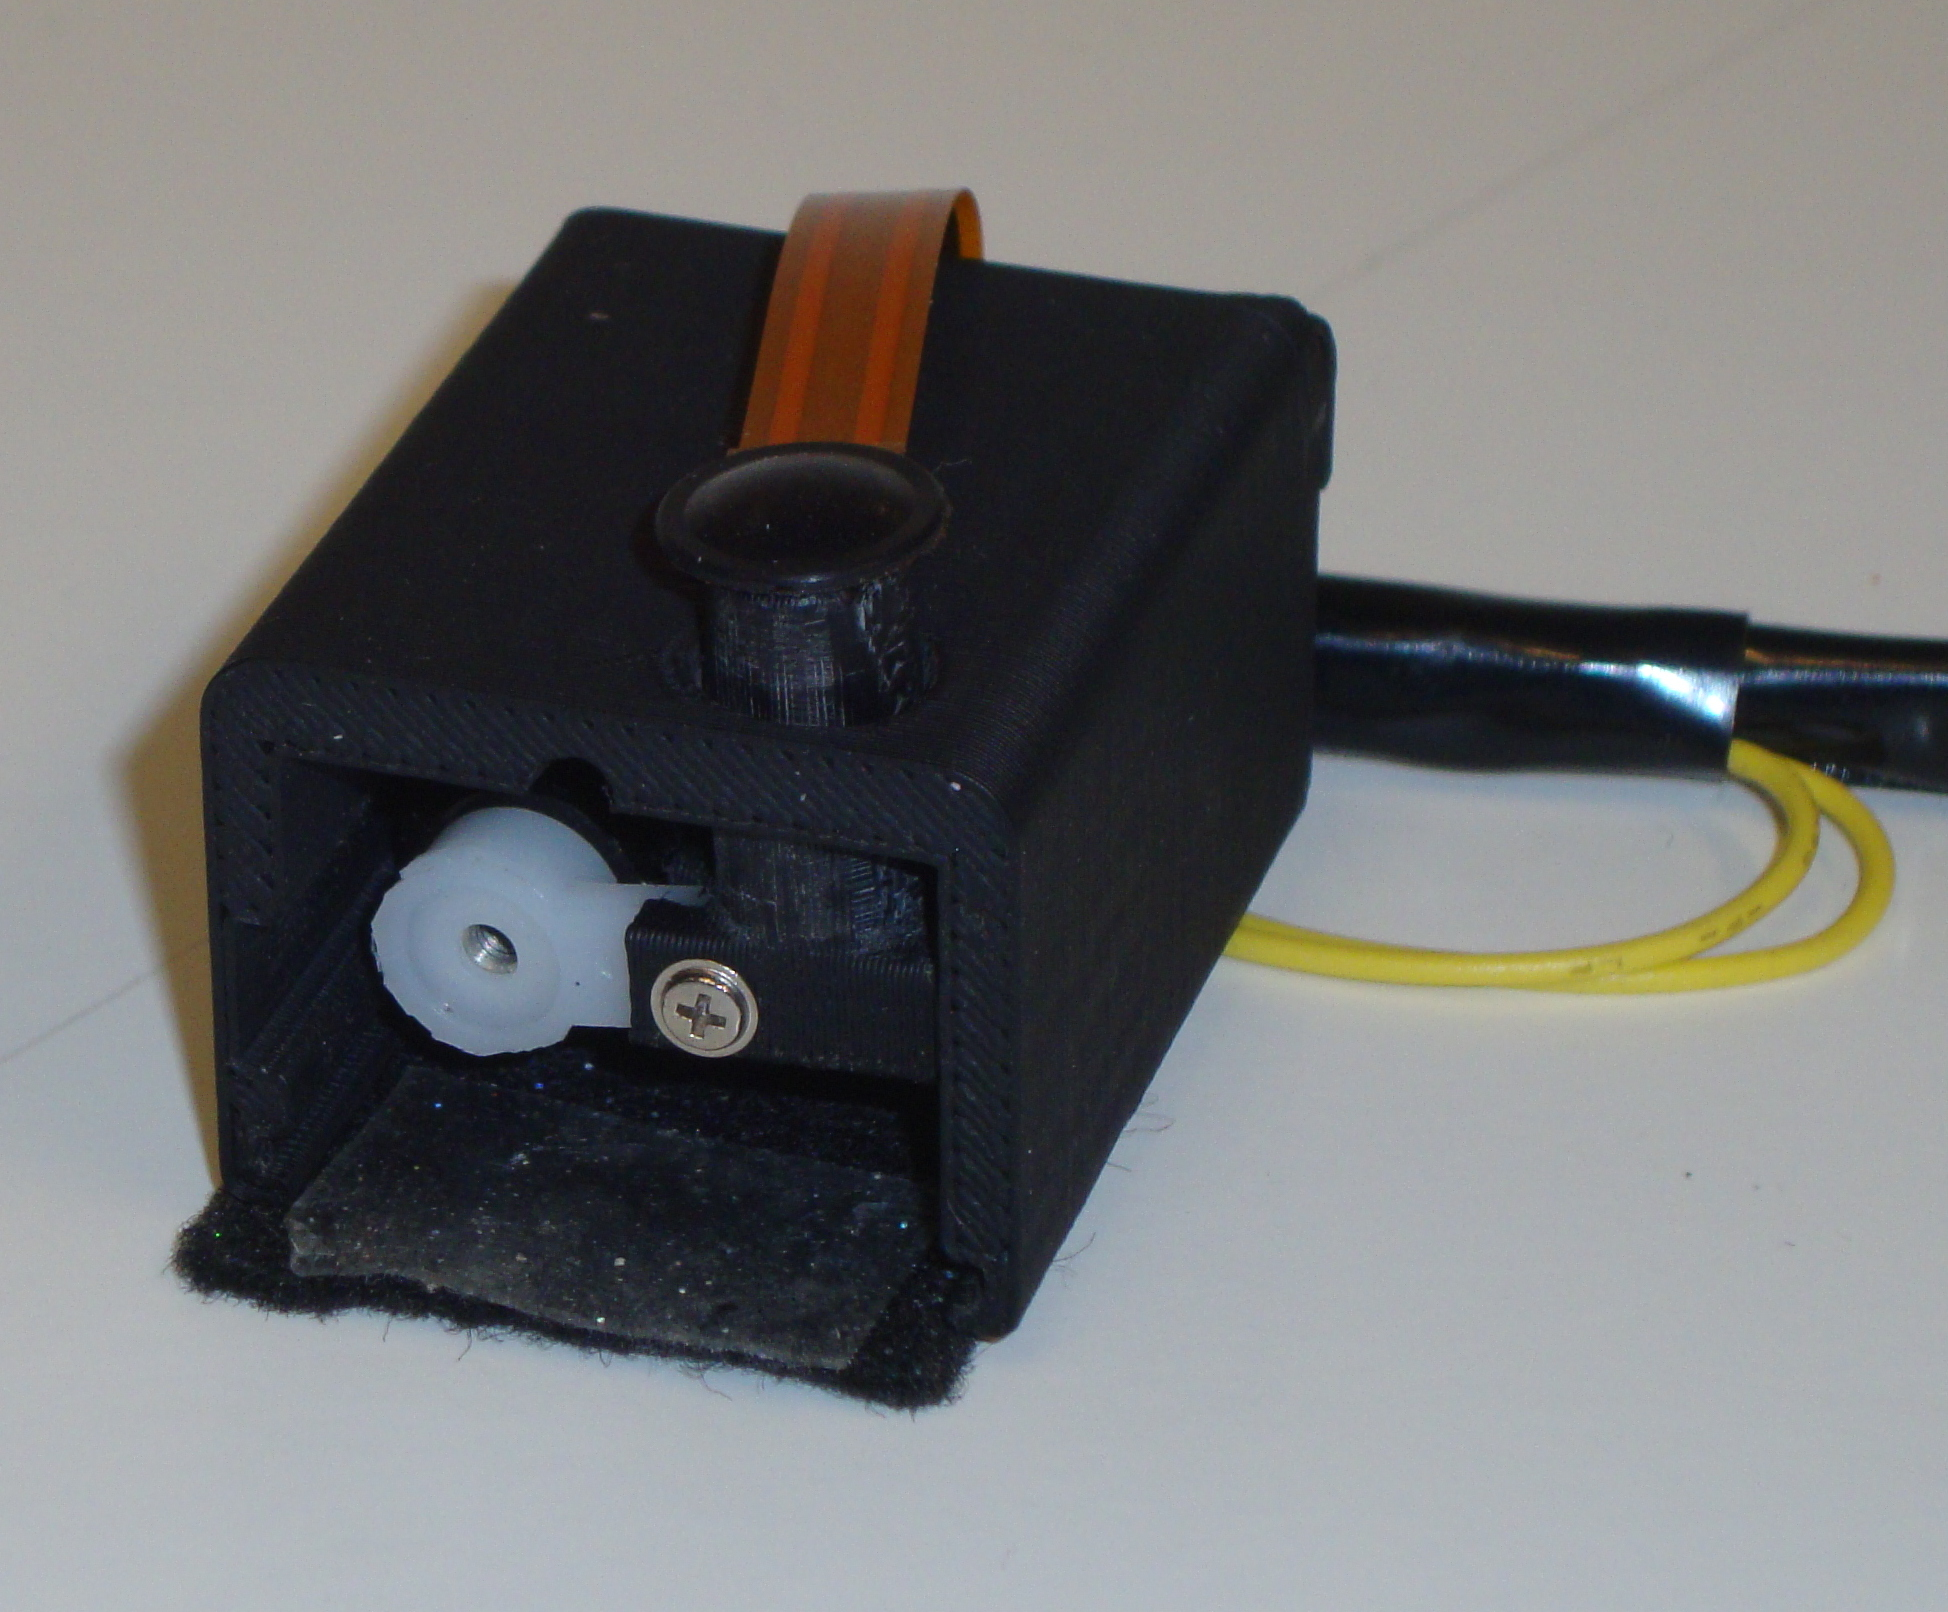
\includegraphics[width=\textwidth,height=\textwidth]{htp2.JPG}
                \caption{HTP}
                \label{fig:Mechanics HTP}
        \end{subfigure}%
        ~ %add desired spacing between images, e. g. ~, \quad, \qquad etc.
          %(or a blank line to force the subfigure onto a new line)
        \begin{subfigure}[H]{0.3\textwidth}
                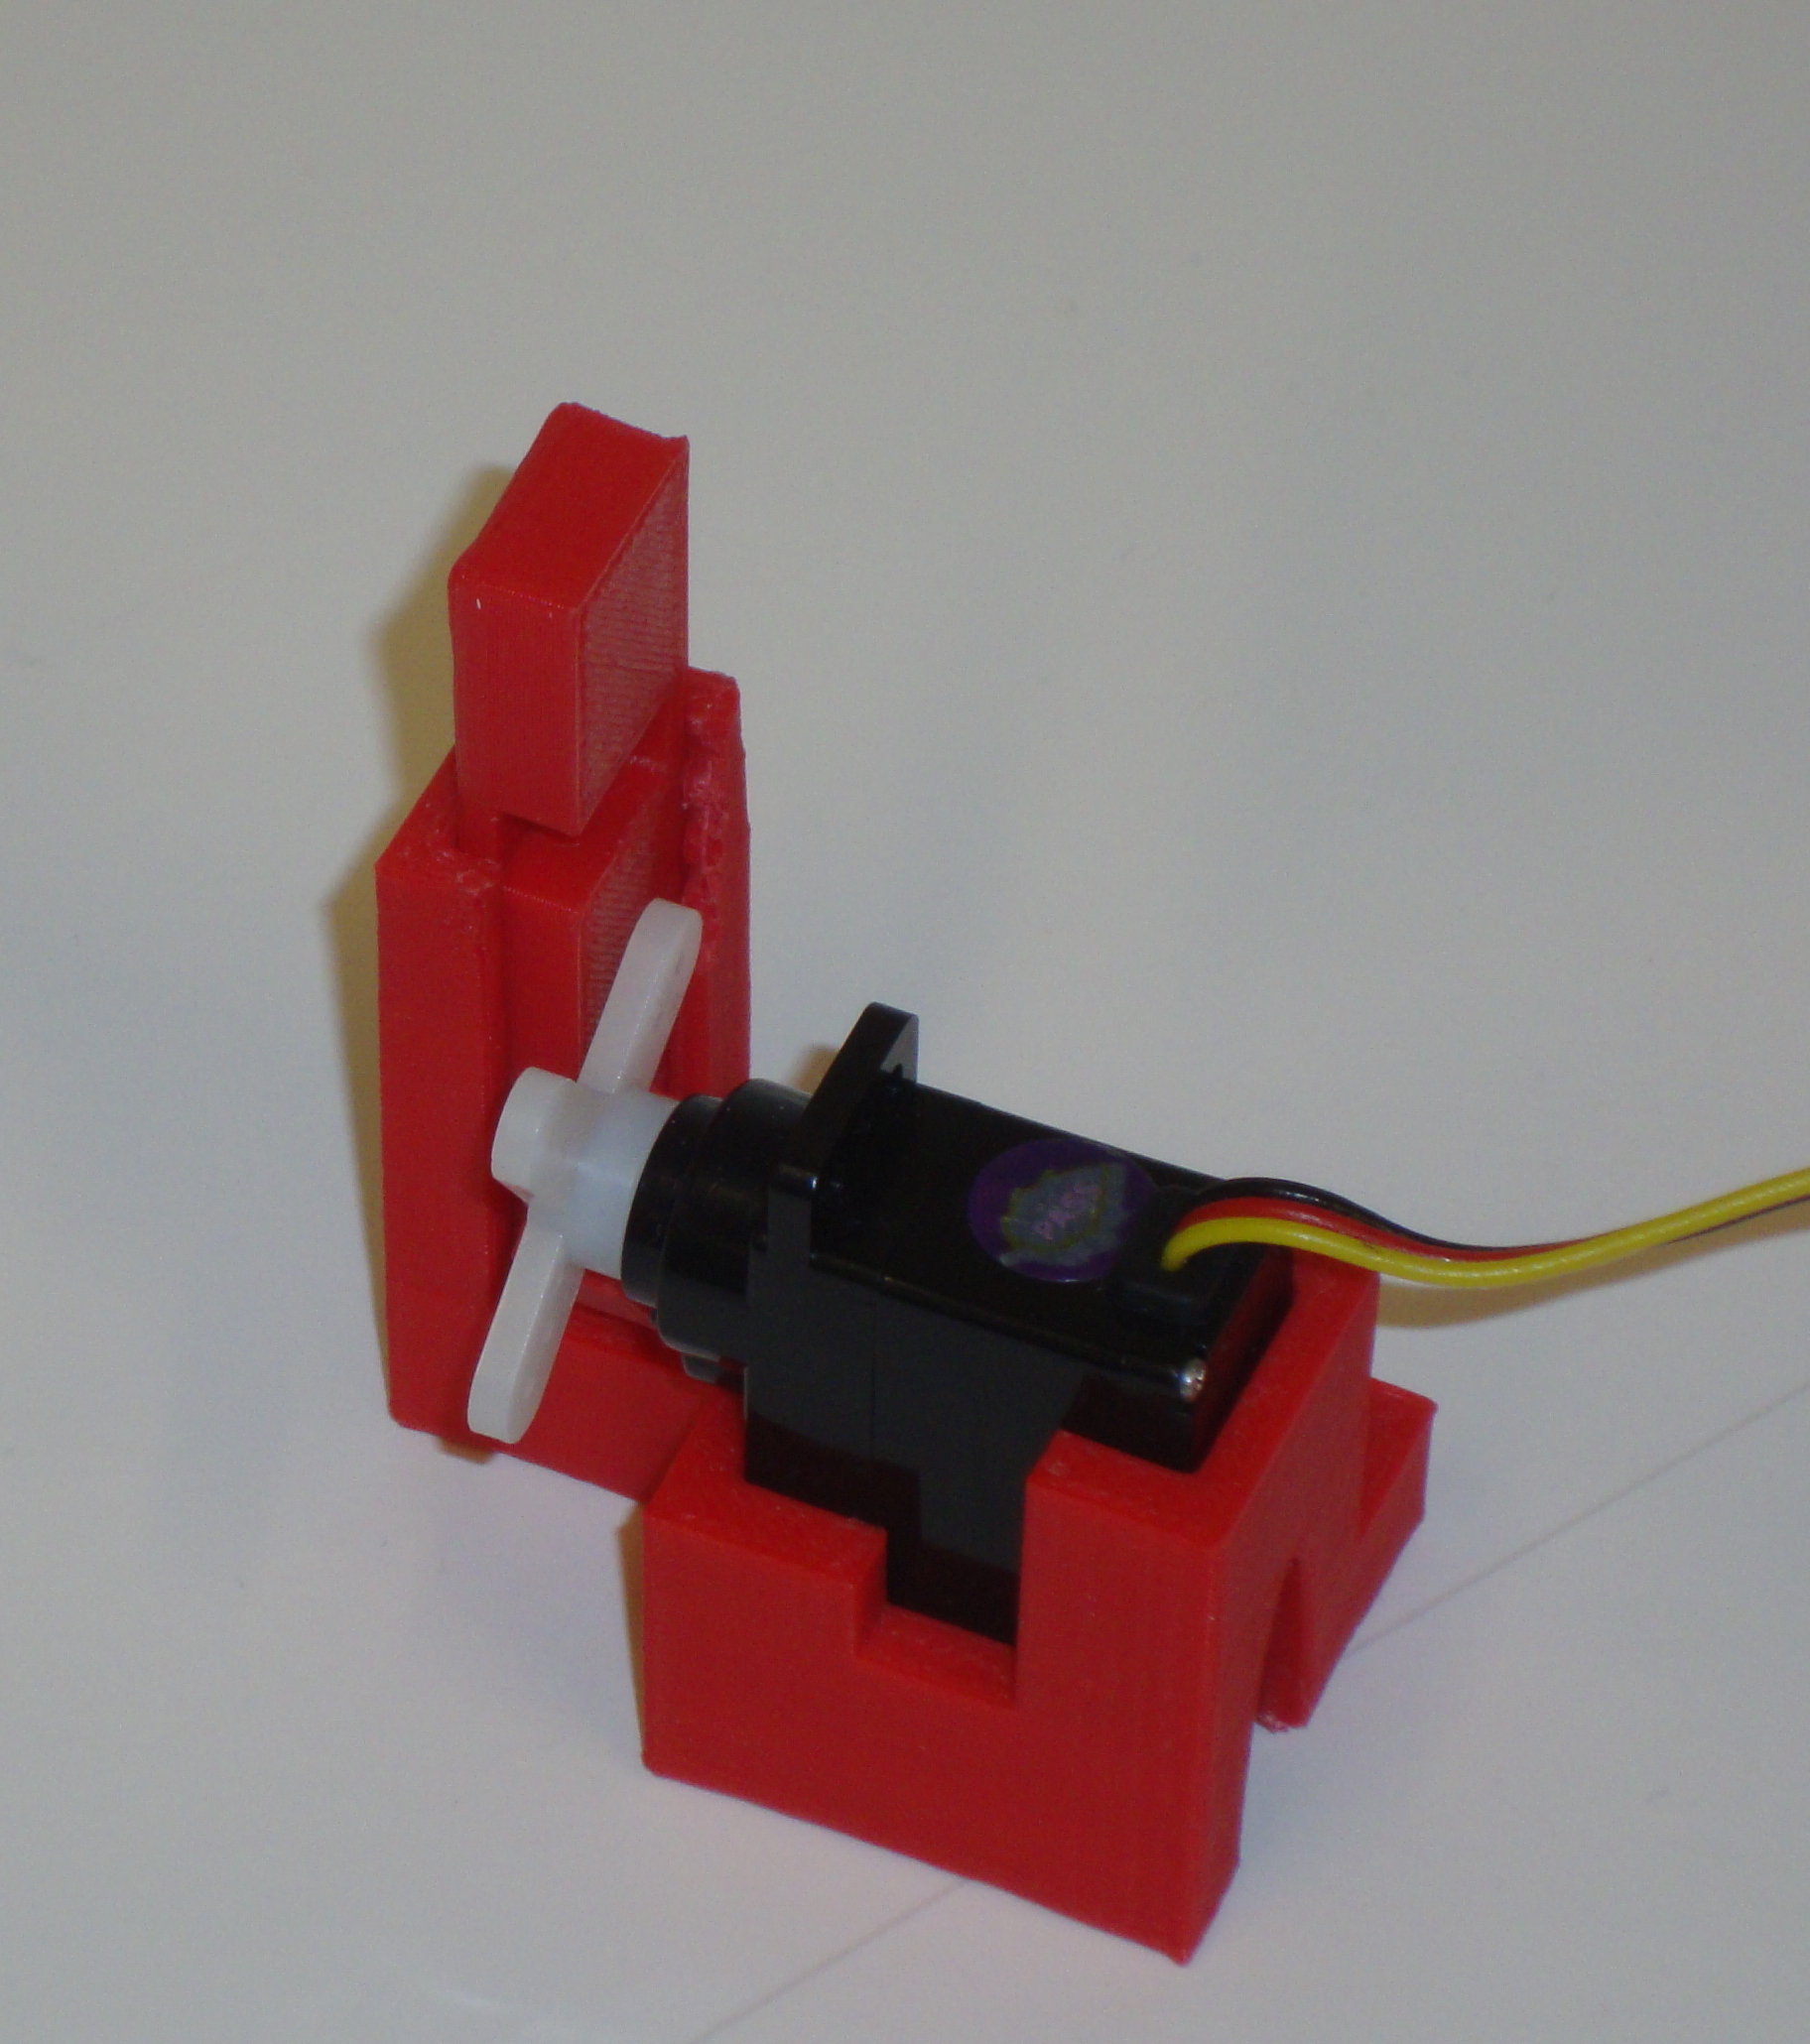
\includegraphics[width=\textwidth,height=\textwidth]{pos1.JPG}
                \caption{HaptiQ MinPos}
                \label{fig:HaptiQ MinPos}
        \end{subfigure}
        ~ %add desired spacing between images, e. g. ~, \quad, \qquad etc.
          %(or a blank line to force the subfigure onto a new line)
        \begin{subfigure}[H]{0.3\textwidth}
                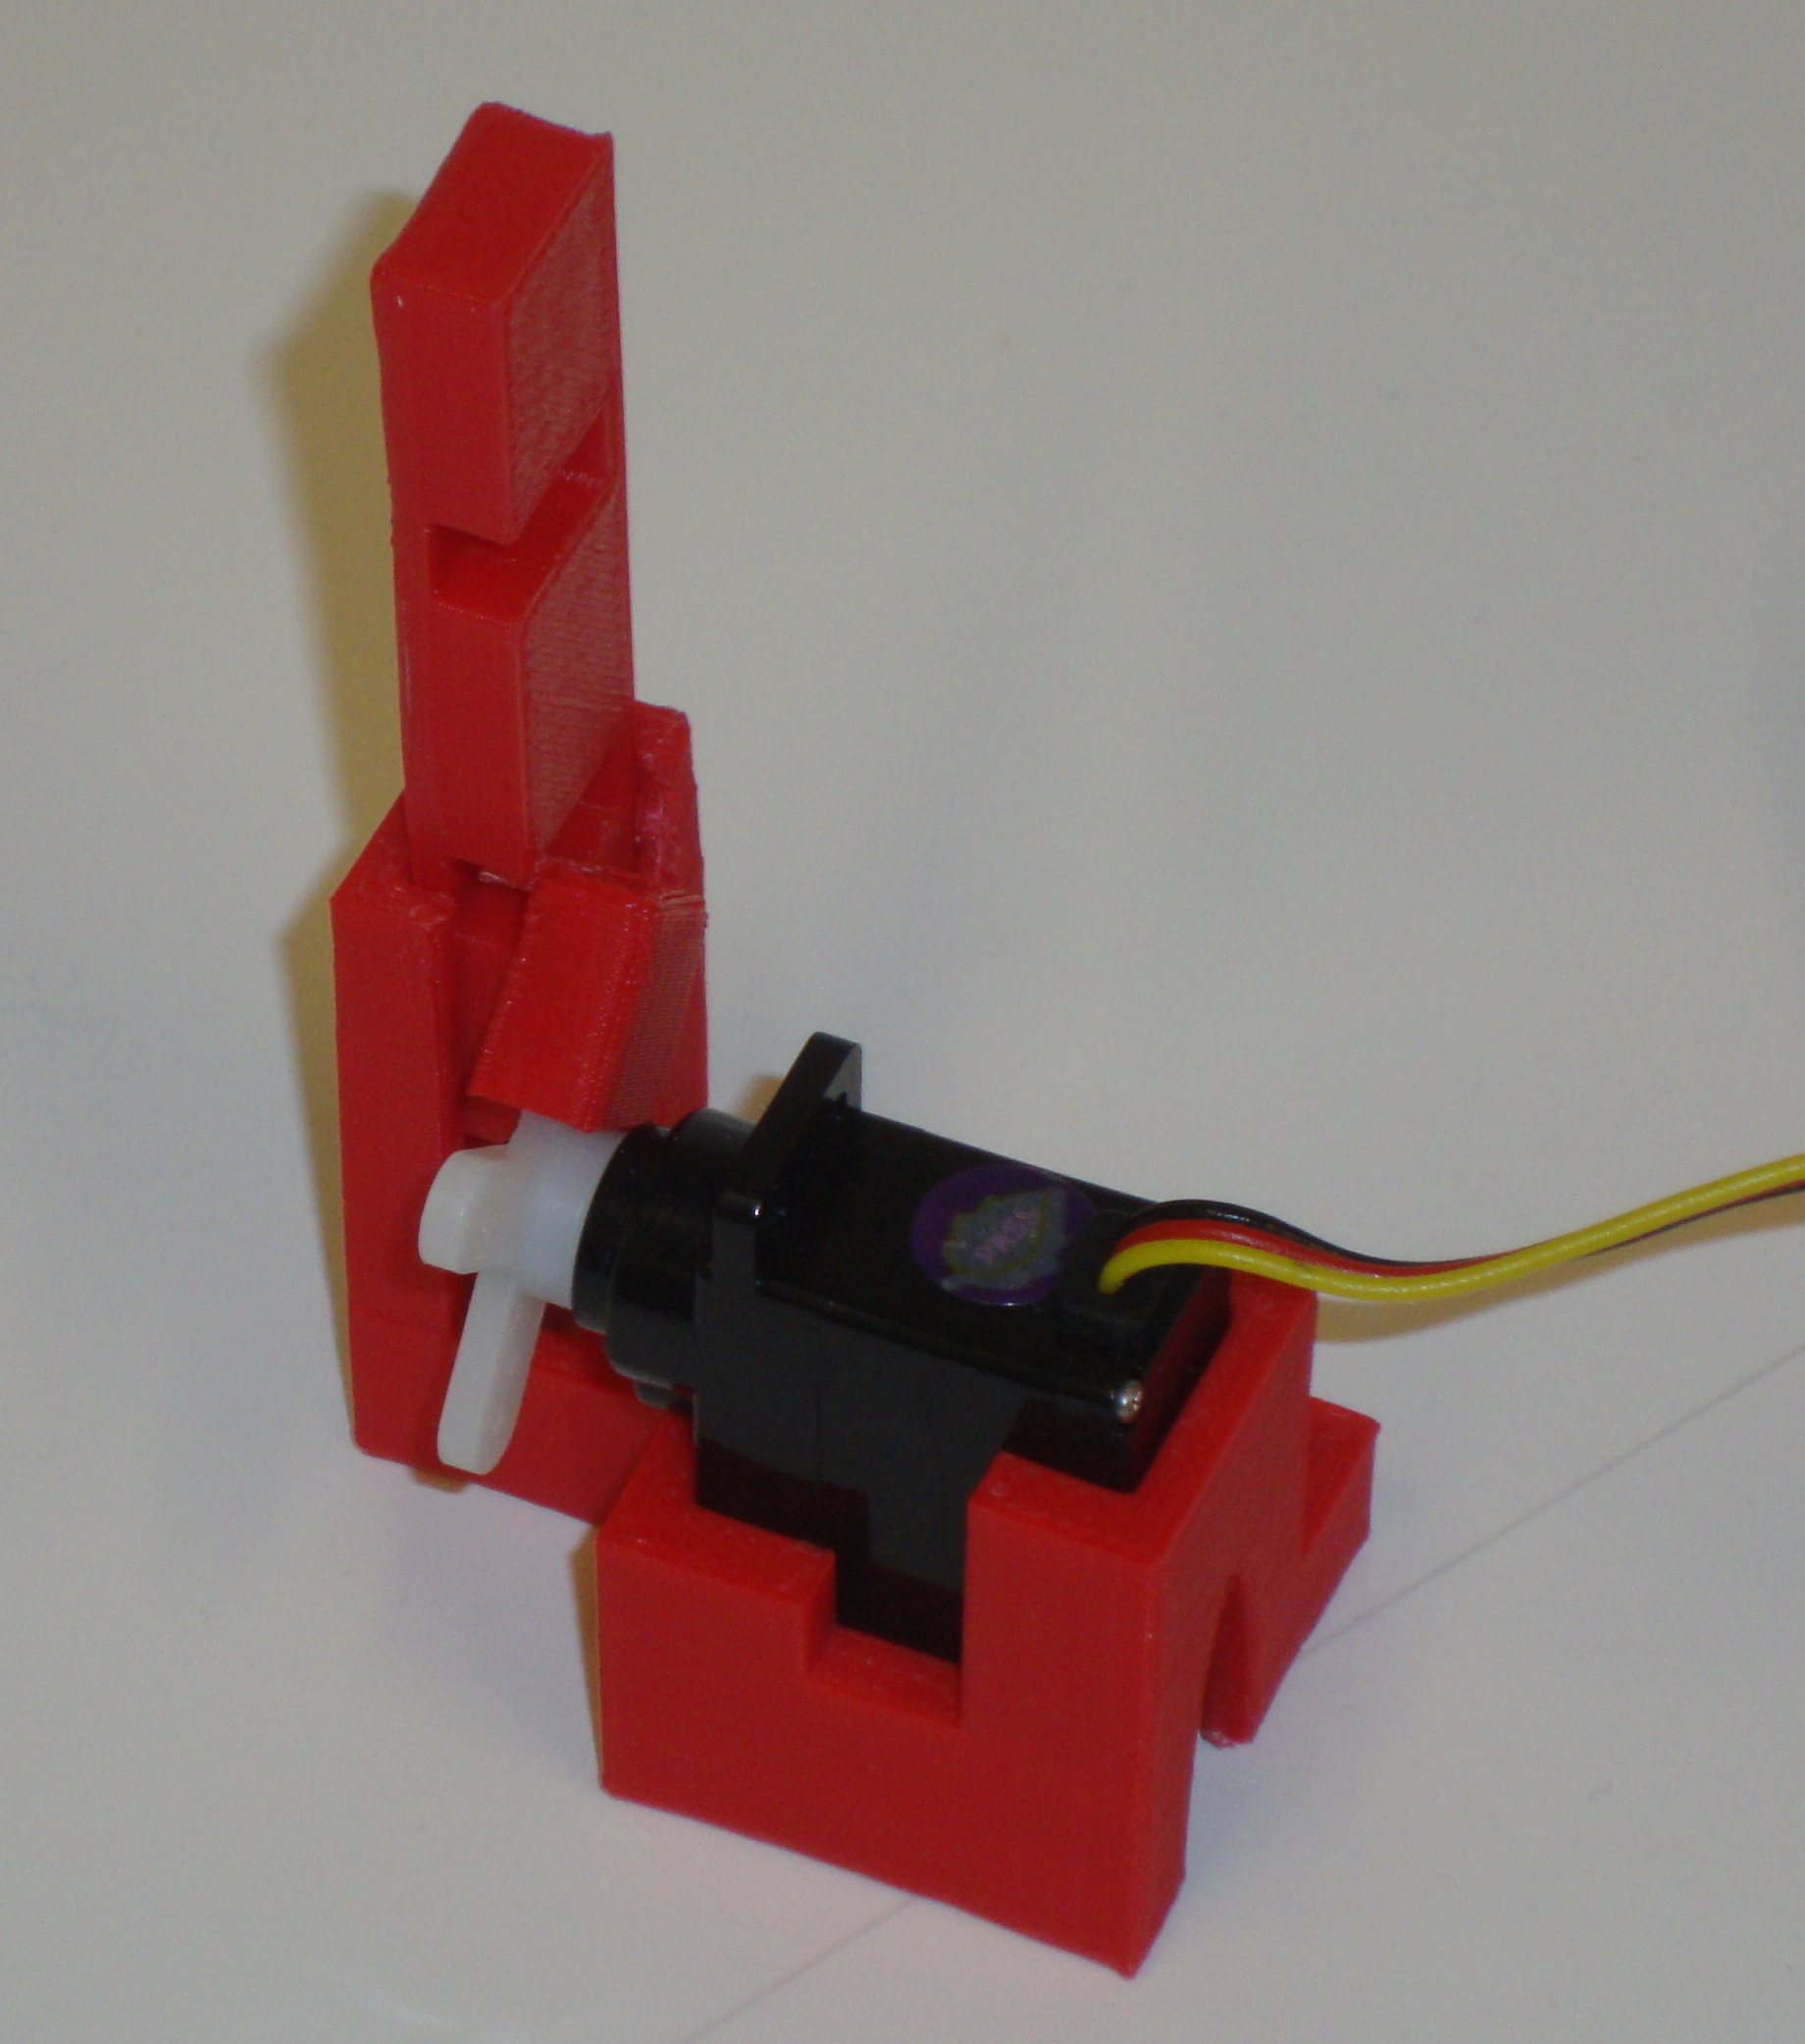
\includegraphics[width=\textwidth,height=\textwidth]{pos2.JPG}
                \caption{HaptiQ MaxPos}
                \label{fig:HaptiQ MaxPos}
        \end{subfigure}
        \caption{HTP and HaptiQ actuator mechanics}\label{fig:HTP and HaptiQ actuator mechanics}
\end{figure}

This version of the HaptiQ does not provide any case. The uneven surface leads to the lack of a reference point or plane for the actuators. This is a major problem in cases where the actuators change position while the user is not currently laying his hand on the device. In fact, it follows that when the blind user places the hand on top of the device again, he or her is not able to tell what the current state of the actuators is compared to the previous one. Two solutions are provided for the 4-HaptiQ: a mid-point reference and a plane reference static actuators (see Figure ~\ref{fig:HaptiQ reference static actuators}). It is not clear which type of reference actuator works best though. My hypothesis is that the plane reference actuator should be more comfortable when using the device and provides the same functionality than the point reference actuator. 

\begin{figure}
        \centering
        \begin{subfigure}[H]{0.5\textwidth}
                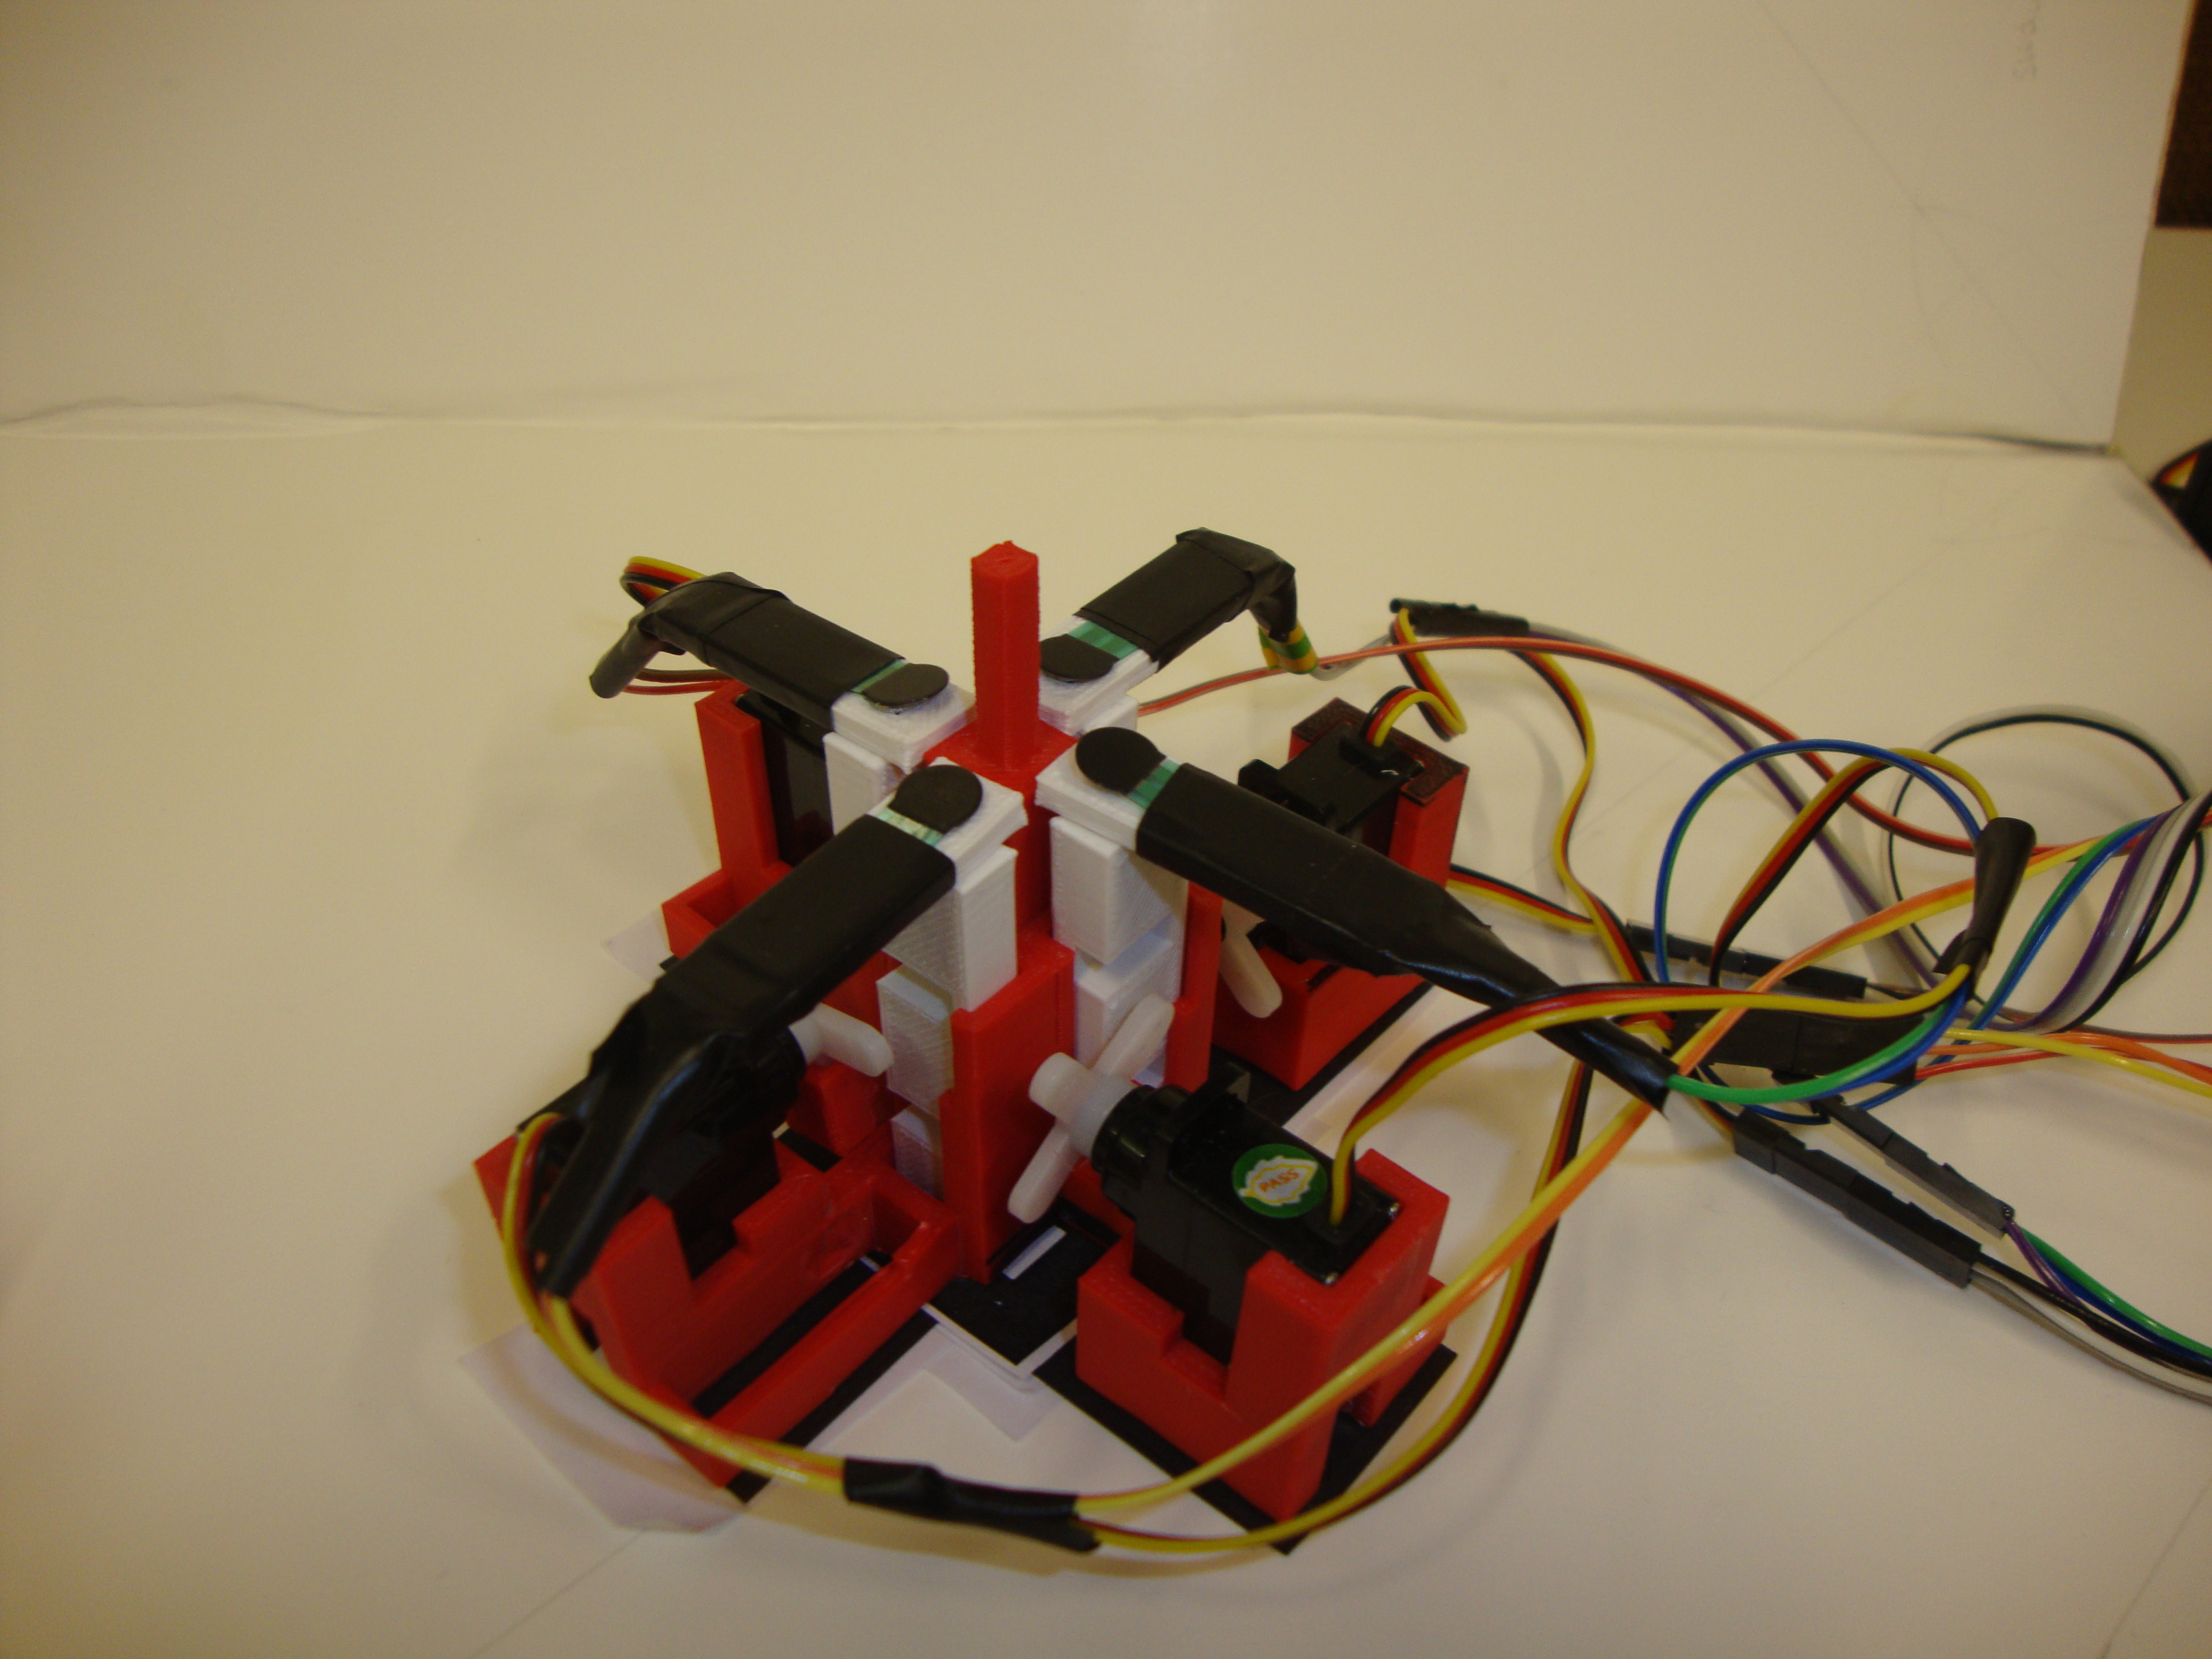
\includegraphics[width=\textwidth]{referencetype20.JPG}
                \caption{Mid-Point reference actuator}
                \label{fig:Mid-Point reference actuator}
        \end{subfigure}%
        ~ %add desired spacing between images, e. g. ~, \quad, \qquad etc.
          %(or a blank line to force the subfigure onto a new line)
        \begin{subfigure}[H]{0.5\textwidth}
                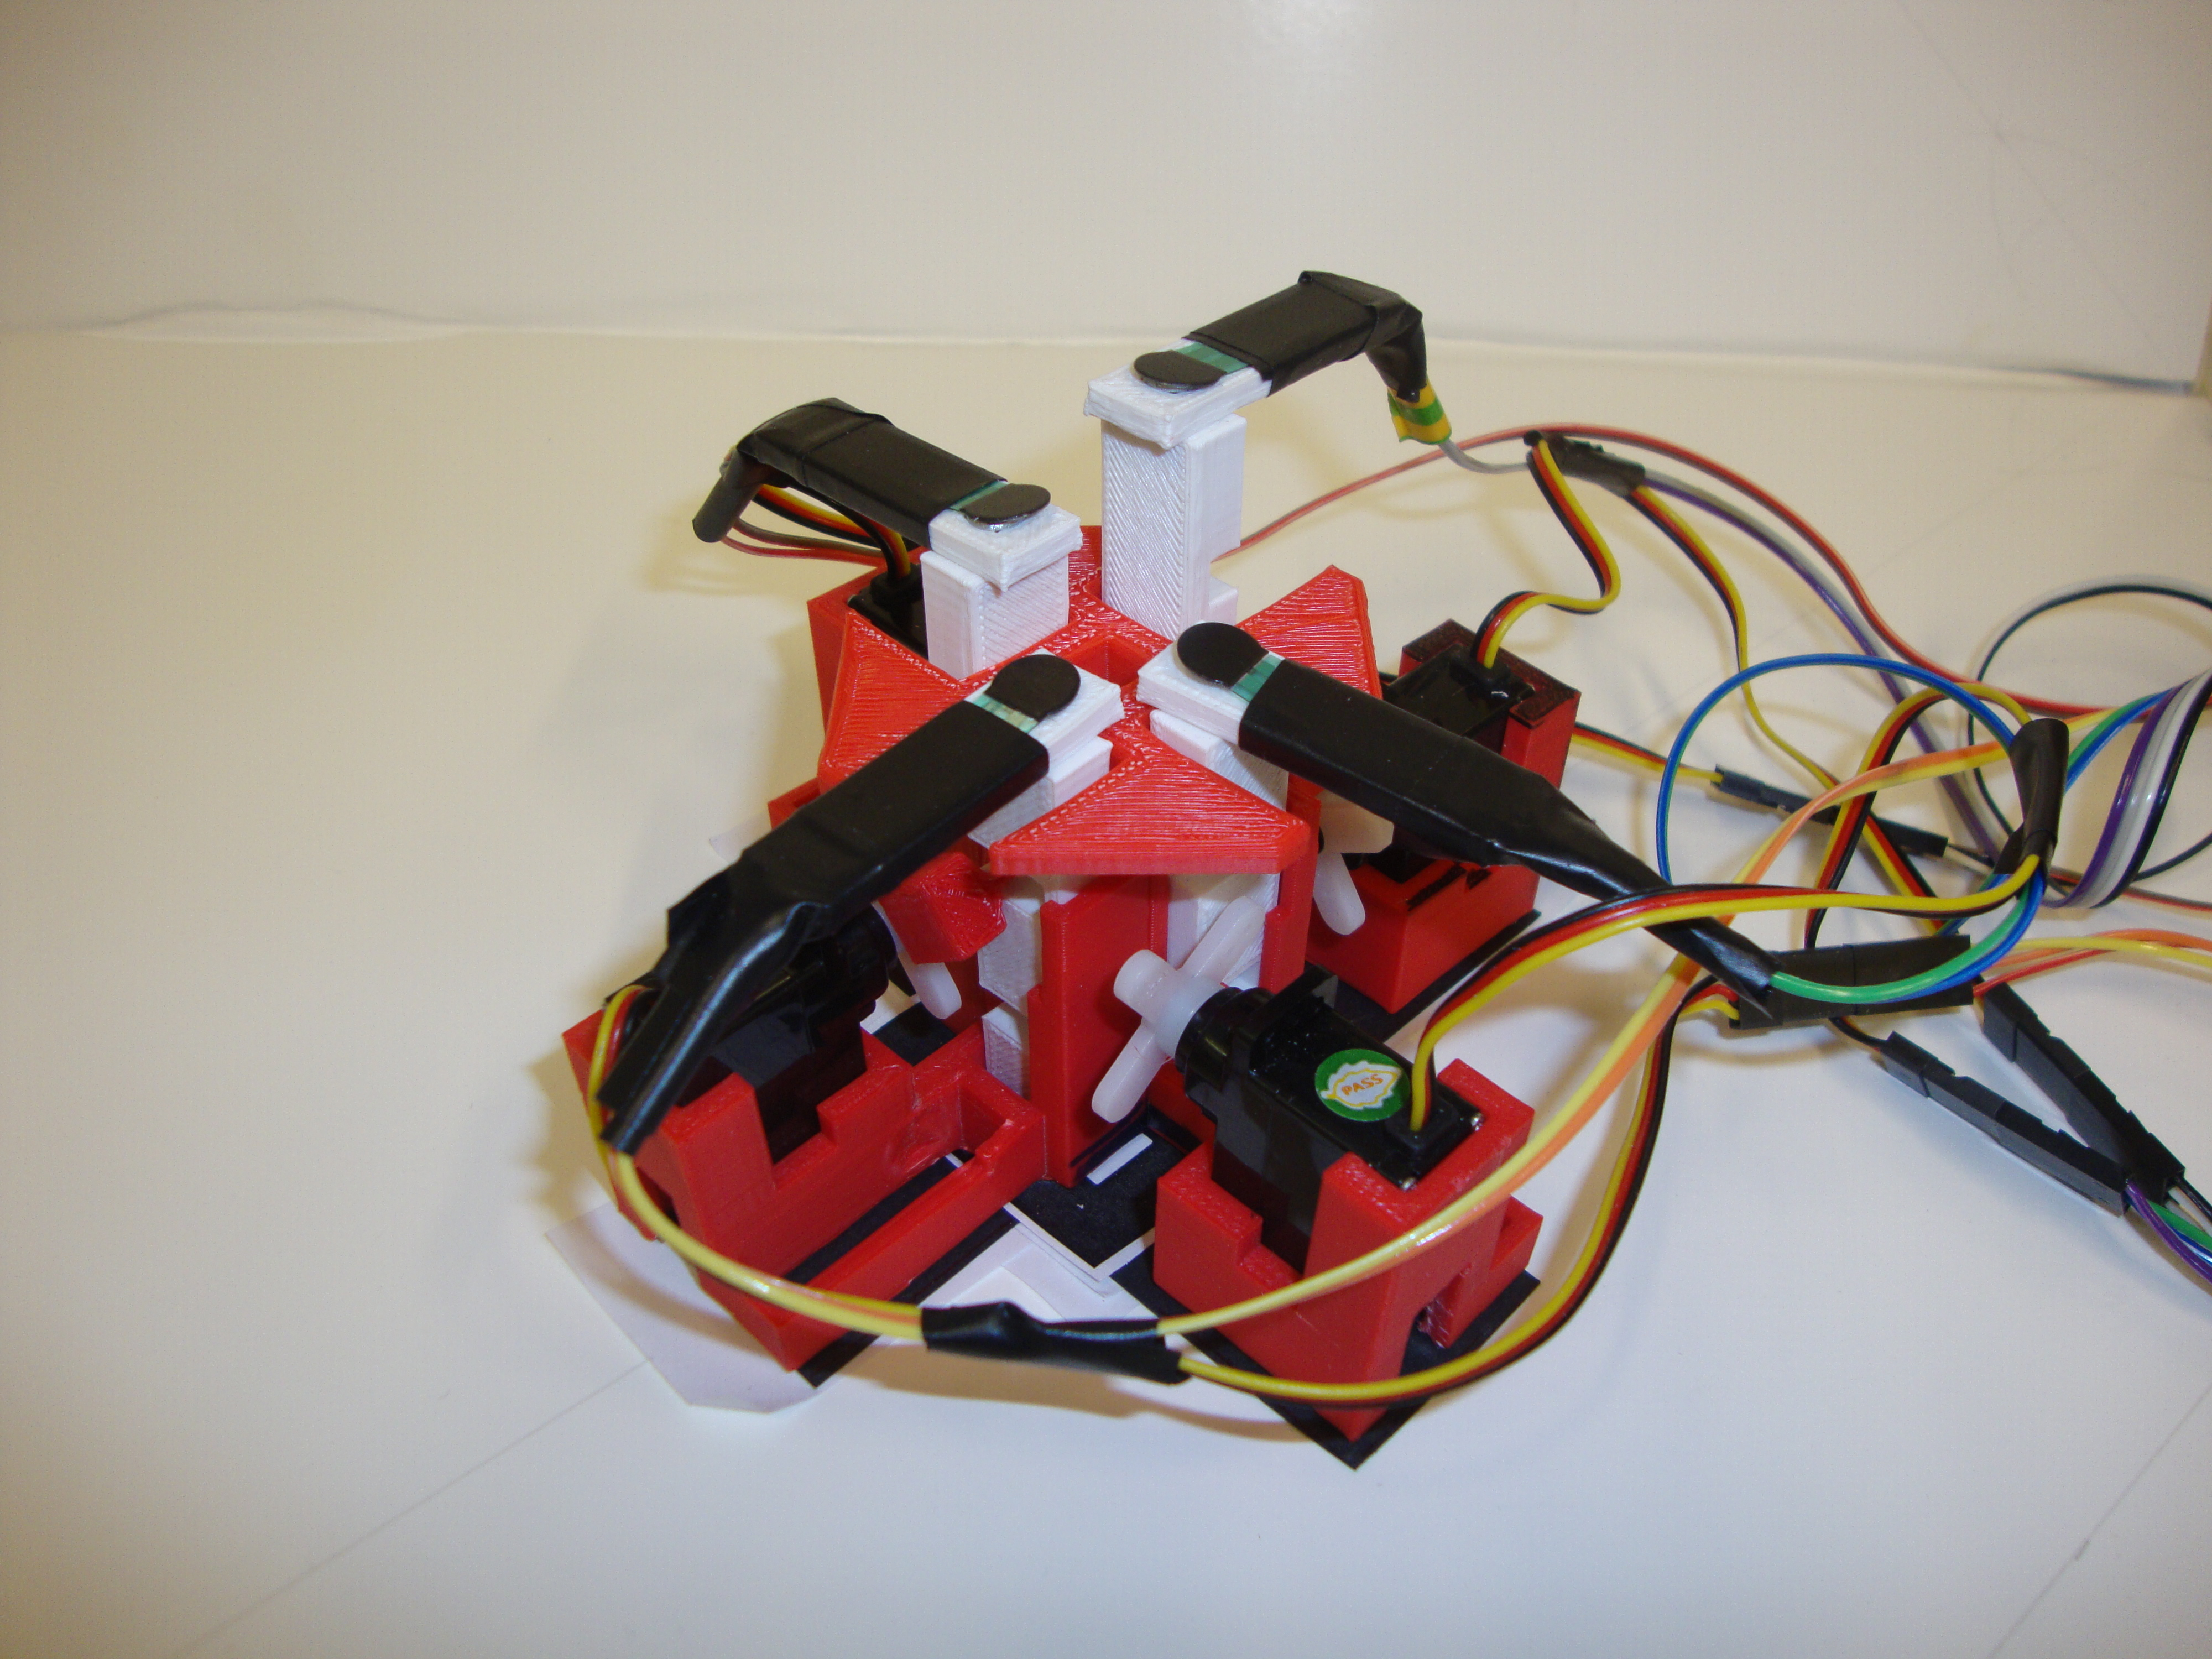
\includegraphics[width=\textwidth]{referencetype11.JPG}
                \caption{Plane reference actuator}
                \label{fig:Plane reference actuator}
        \end{subfigure}
        ~ %add desired spacing between images, e. g. ~, \quad, \qquad etc.
        \caption{HaptiQ reference static actuators}\label{fig:HaptiQ reference static actuators}
\end{figure}

The HaptiQ is the first vector-based display for blind users. Whether this design provides better feedback to users or not is unknown, because no study with participants could be conducted. Therefore, the actuators are designed so to support different tops in order to be able to evaluate the HaptiQ against a point-based haptic feedback TUI. In the version here presented, only vector-like tops are provided, but other type of tops can be easily printed and fasten to the actuators.   

Finally, the HaptiQ does not have any break to simulate friction. While it could be possible to add this feature, I decided that the primary goal of this project was just to focus on the vectorisation of the actuators. 

\subsection{8-HaptiQ}
The result of the final design iteration is the 8-HaptiQ. Using the same design of the 4-HaptiQ for eight actuators would lead to a considerable increase in size of the device. Therefore, the 8-HaptiQ has been completely re-engineered (see Figure ~\ref{fig:8-HaptiQ}). 

\begin{figure}[H]
  \centering
  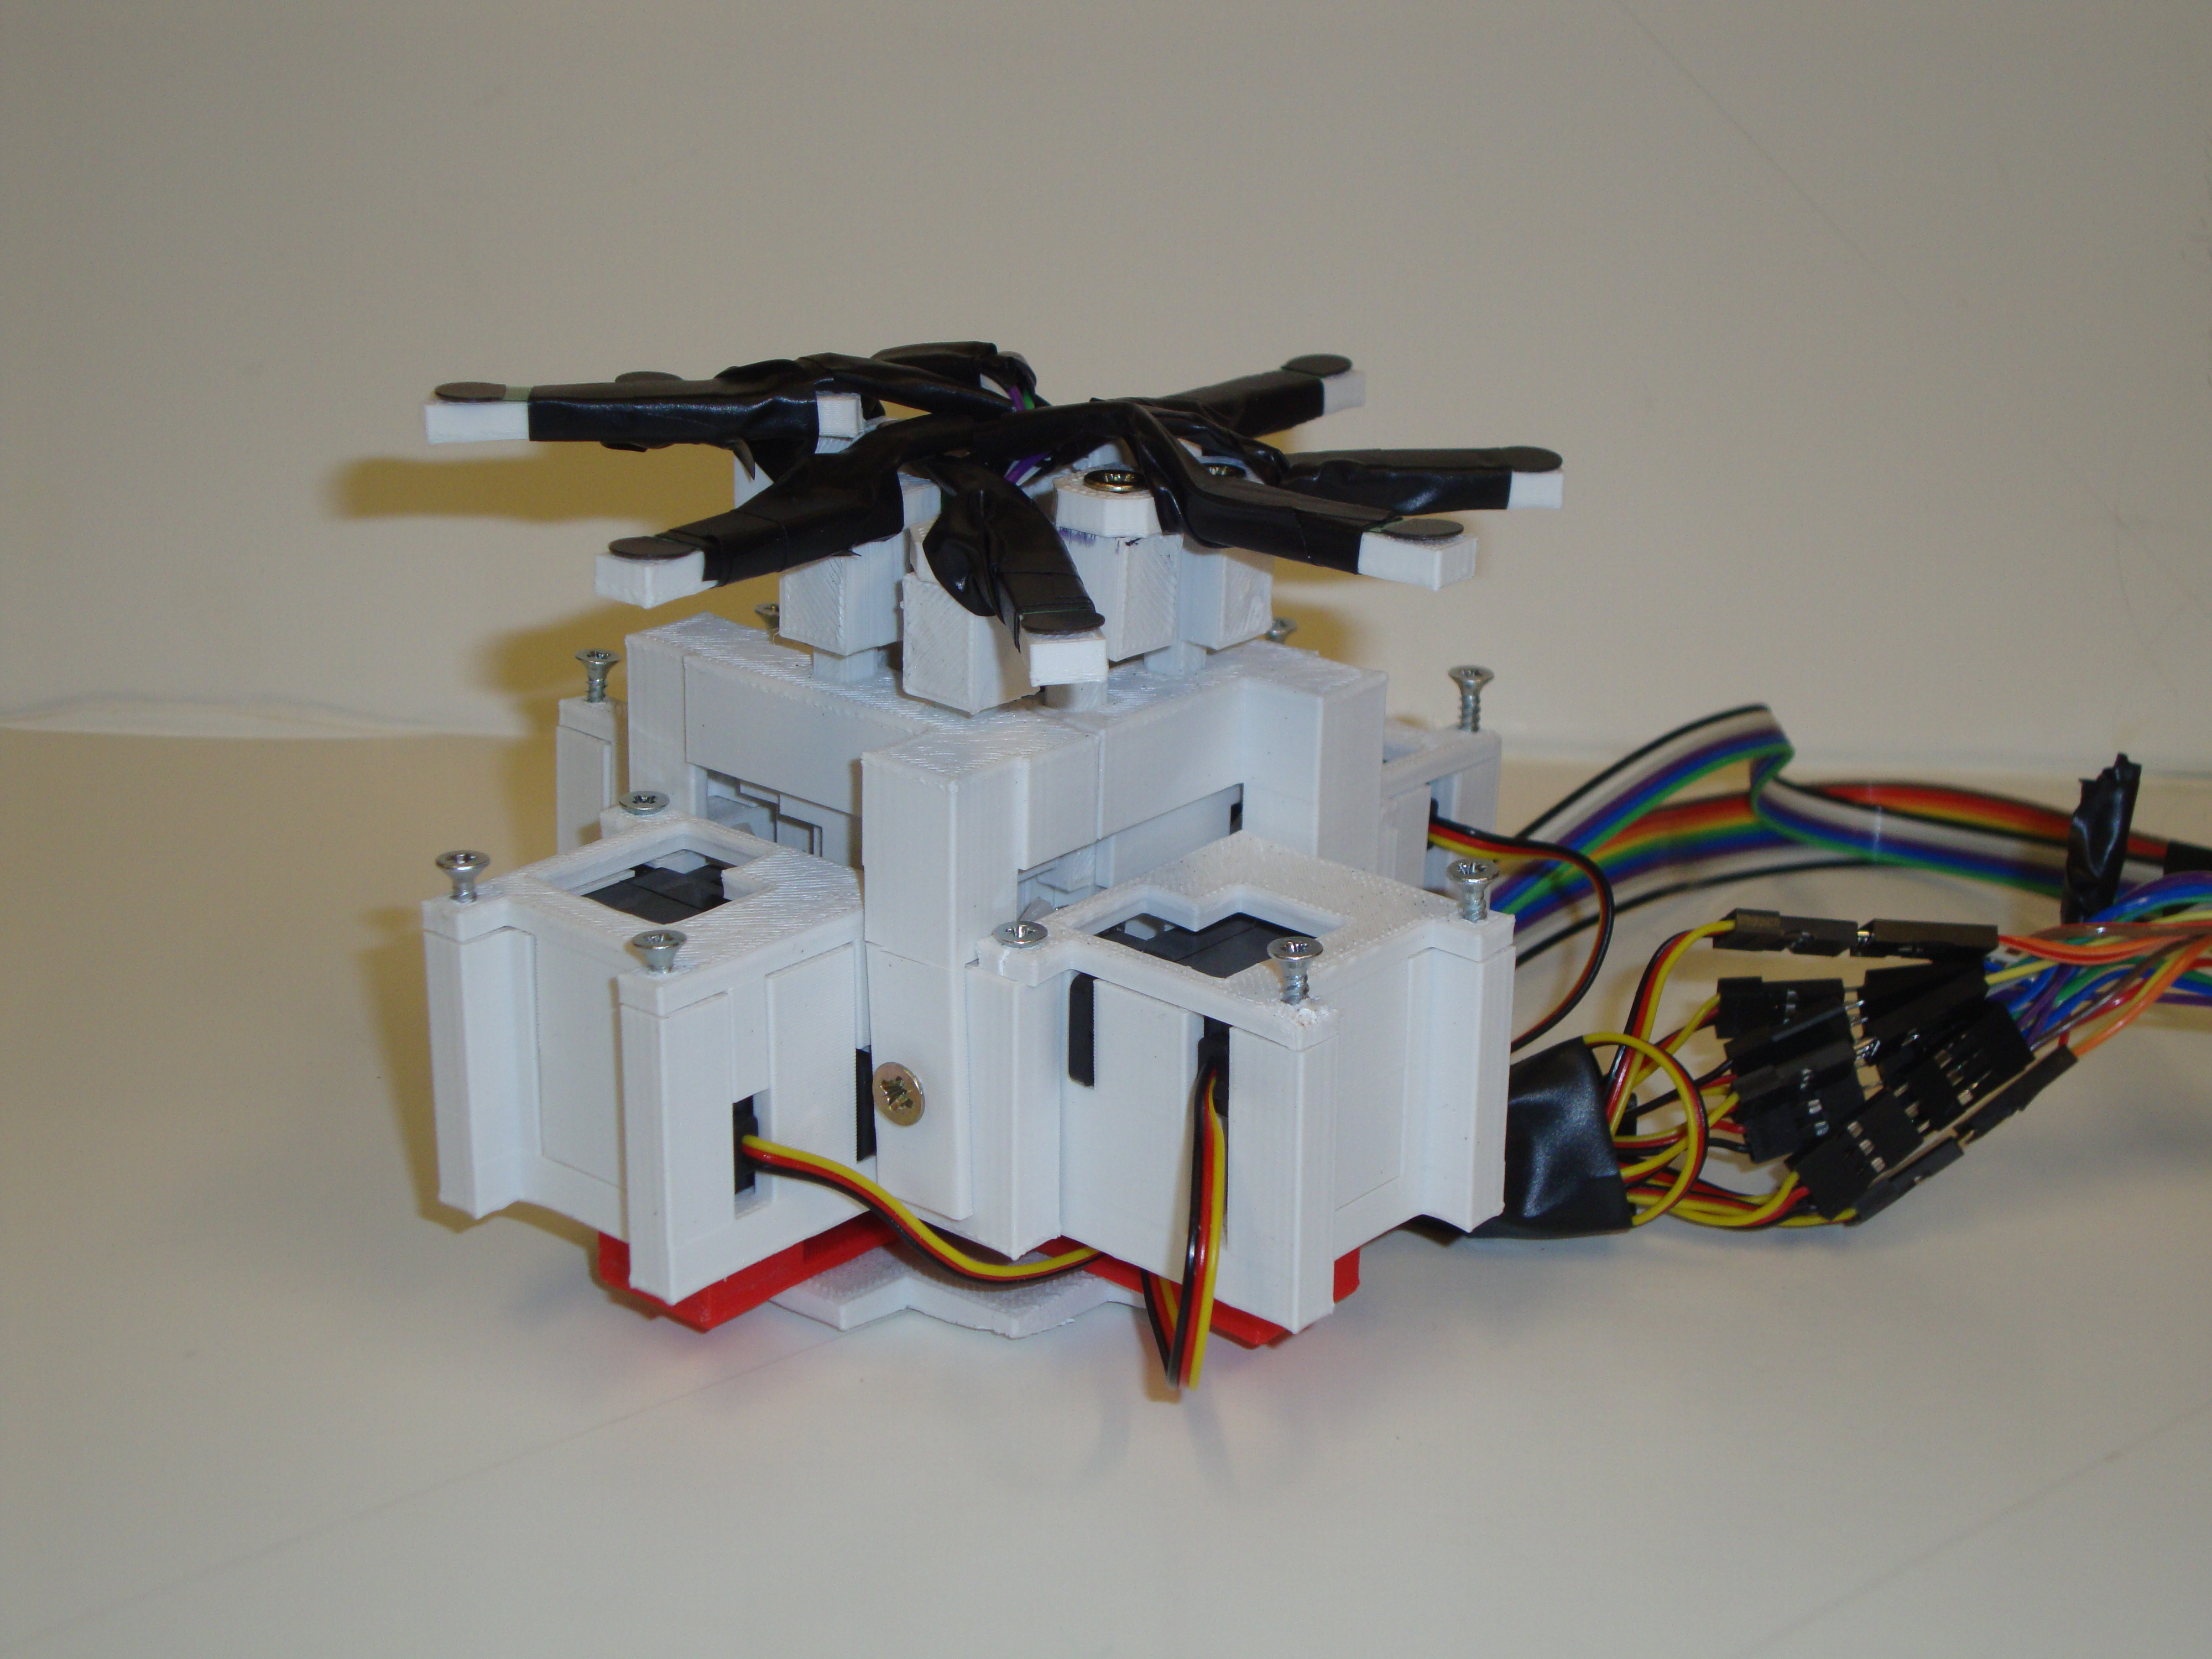
\includegraphics[width=0.7\textwidth]{HaptiQ1.JPG}
  \caption{8-HaptiQ}
  \label{fig:8-HaptiQ}
\end{figure}

The 4-HaptiQ not only is not optimised in terms of space, but its wiring is also not well engineered. As it is possible to observe in Figure ~\ref{fig:HaptiQ reference static actuators} the wiring does not allow the device to be used comfortably, especially when one wants to rotate it. 
The servos in the 8-HaptiQ are organised in couples. Unlike its predecessor, the servos are positioned horizontally (see Figure ~\ref{fig:8-HaptiQservos}) and the screws are moved more toward the center of rotatory mechanism of the servos. These design choices allow the device to be more compact and still preserve the same functionalities of the 4-HaptiQ. 
The device is lift up by an additional structure laying below it, allowing the wiring to be less disruptive. 

\begin{figure}[H]
  \centering
  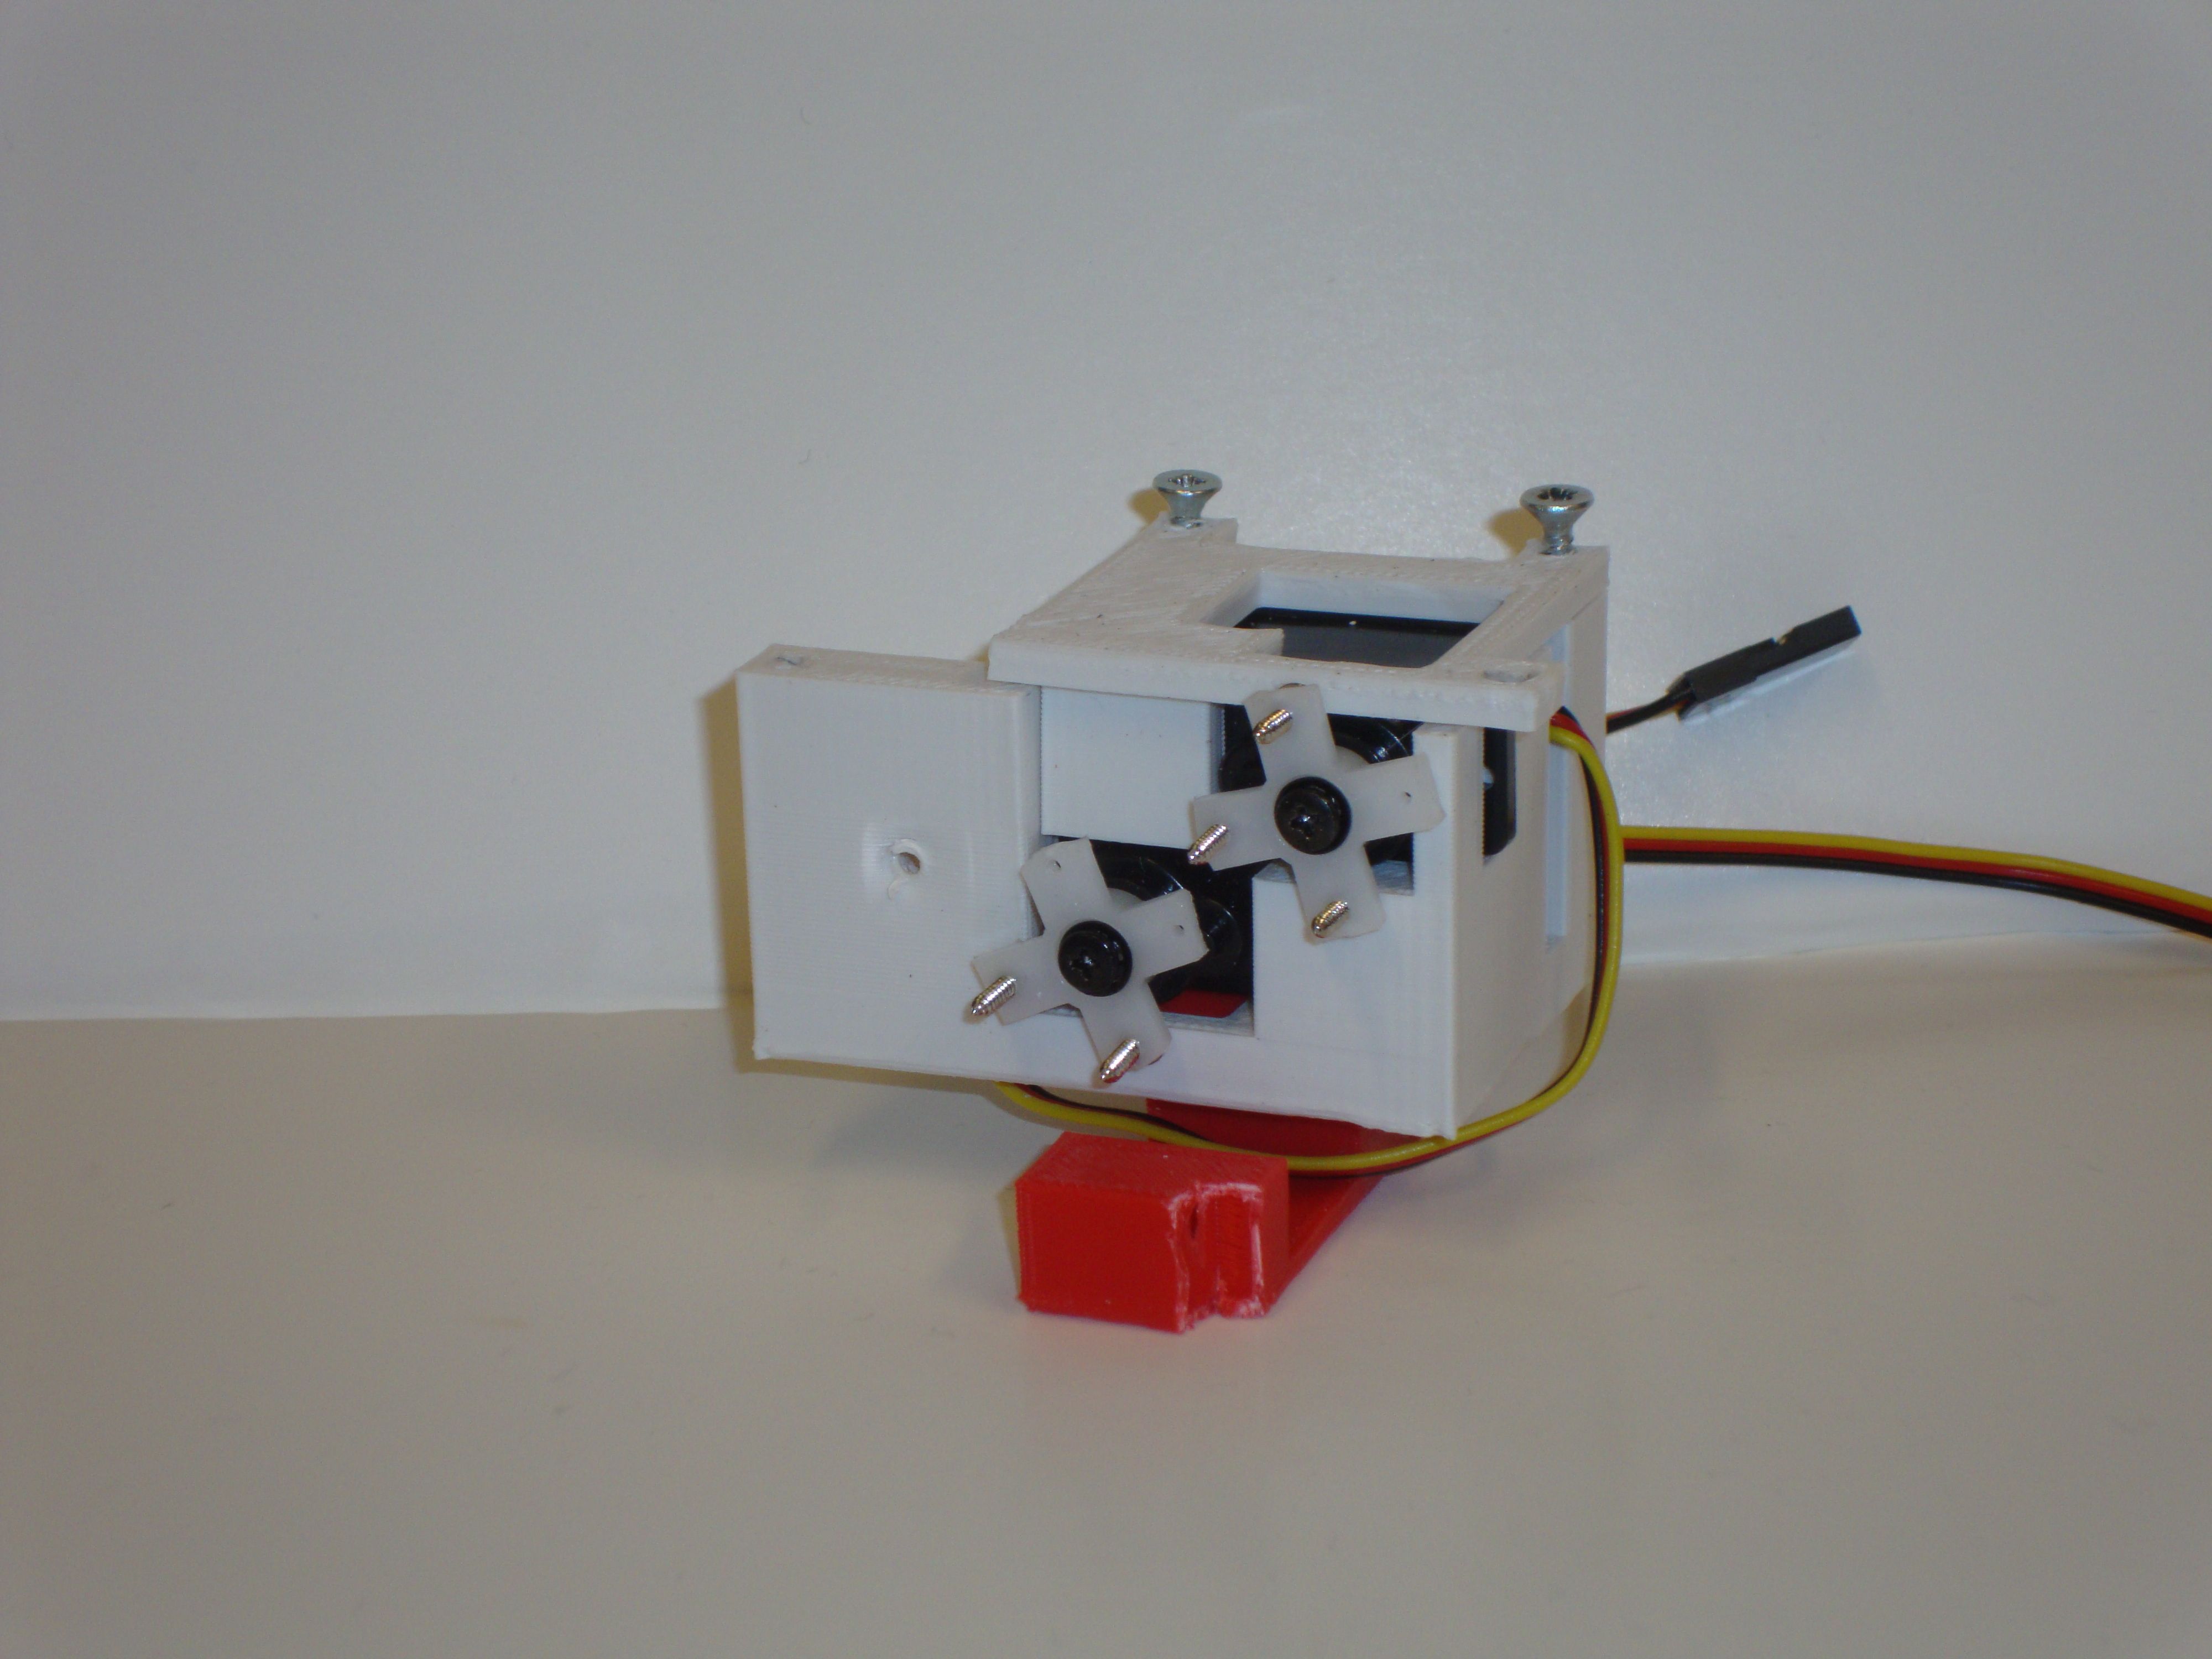
\includegraphics[width=0.7\textwidth]{8haptiQservos.JPG}
  \caption{8-HaptiQ servos couple}
  \label{fig:8-HaptiQservos}
\end{figure}

With the gathering of the wires for the sensors to the center of the device, the position of the sensors is also inverted compared to the 4-HaptiQ. While in the 4-HaptiQ the sensors meet in the middle, with this new version of the HaptiQ they are spread to the outside. It is not clear whether this design choice is an advantage or not in terms of usability. Alternatives to this solution will be provided in the near future, as discussed in the Future Work chapter.

The 8-HaptiQ takes a different approach for the design of the actuators guides. In the first version, a base was provided for the actuator, which limits this to move further down when this is at its minimum position (see Figure ~\ref{fig:HaptiQ MinPos}). But to provide an optimal wiring, the 8-HaptiQ combines the guides for all the actuators with the reference plane (see Figure ~\ref{fig:8haptiqref}). Additional connecting screws allow the actuators to be always controlled by the servos and not to fall below its minimum position. 

\begin{figure}[H]
  \centering
  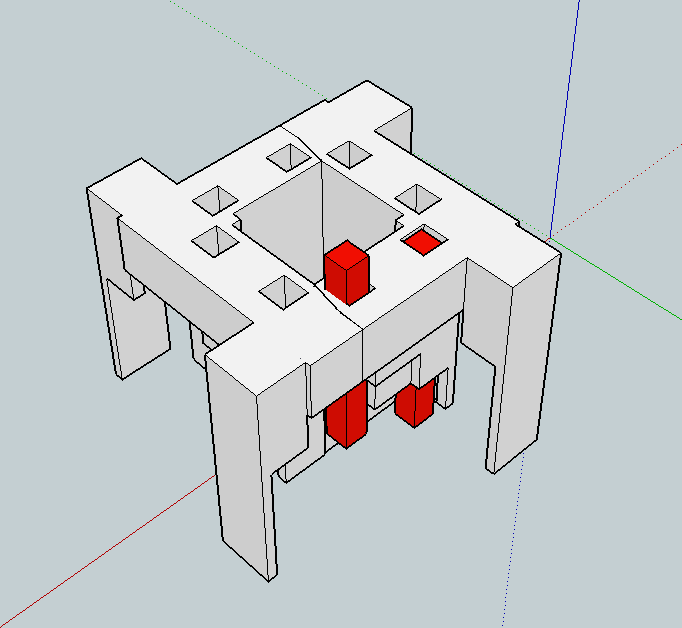
\includegraphics[width=0.6\textwidth]{8HaptiQSlots2.png}
  \caption{8-HaptiQ reference plane and actuators slots}
  \label{fig:8haptiqref}
\end{figure}

\subsection{Fiducial Markers}

The HaptiQ, like the HTP, is designed to work on interactive tabletops. Specifically on Microsoft PixelSense tables (supporting Microsoft Surface SDK 2.0) \cite{pixelsense}. The Microsoft Surface Bytetag is the standard fiducial marker for the PixelSense tables (see Figure ~\ref{fig:Bytetag}). But Bytetags are hard to print, if high accuracy is wanted, and expensive, if one wants to buy them from the official store.

The HaptiQ, in addition to the  Microsoft Bytetags, supports Glyph, as defined by the Glyph Recognition And Tracking Framework (GRATF) (see Figure ~\ref{fig:glyph}).

Both types of fiducial markers are to be displaced on the bottom of the device, if a PixelSense table (or equivalent) is used. Otherwise, it could be possible to place a Glyph on top of the device, provided that an appropriate structure is built, and recognise it using a web-cam. 

\begin{figure}[H]
        \centering
        \begin{subfigure}[H]{0.3\textwidth}
                
\includegraphics[width=\textwidth]{bytetag.jpg}
                \caption{Bytetag}
                \label{fig:Bytetag}
        \end{subfigure}%
        ~ %add desired spacing between images, e. g. ~, \quad, \qquad etc.
          %(or a blank line to force the subfigure onto a new line)
        \begin{subfigure}[H]{0.3\textwidth}
                
\includegraphics[width=\textwidth]{glyph3.png}
                \caption{Glyph}
                \label{fig:glyph}
        \end{subfigure}
        ~ %add desired spacing between images, e. g. ~, \quad, \qquad etc.
        \caption{Fiducial Markers}
        \label{fig:fiducialMarkers}
\end{figure}

\section{The API}

This section discusses the design choices taken for the API of the HaptiQ. The general idea is similar to the HapticTouch toolkit \cite{ledo2012haptictouch}. However, this has been completely redesigned to support:

\begin{itemize}
	\item multiple actuators
    \item multiple pressure sensors
    \item a completely new approach to HapticObjects and HapticBehaviours
    \item actions called when input is received by the user
    \item additional API to get input position of the device from different hardware
\end{itemize}

Each of these will be discussed in the following sections. 

\subsection{Overall Structure}

The API consists of two main components: the HaptiQ API used to control the device and the Input API (see Figure ~\ref{fig:api}). 
The HaptiQ API component is designed to provide high and low access to the HaptiQ. This allows the API to be versatile and to be used by beginner, intermediate and advanced developers. 
The HaptiQ API retrieves the position of the device through the Input API. 

The following two sections describe these components in more details.

\begin{figure}[H]
  \centering
  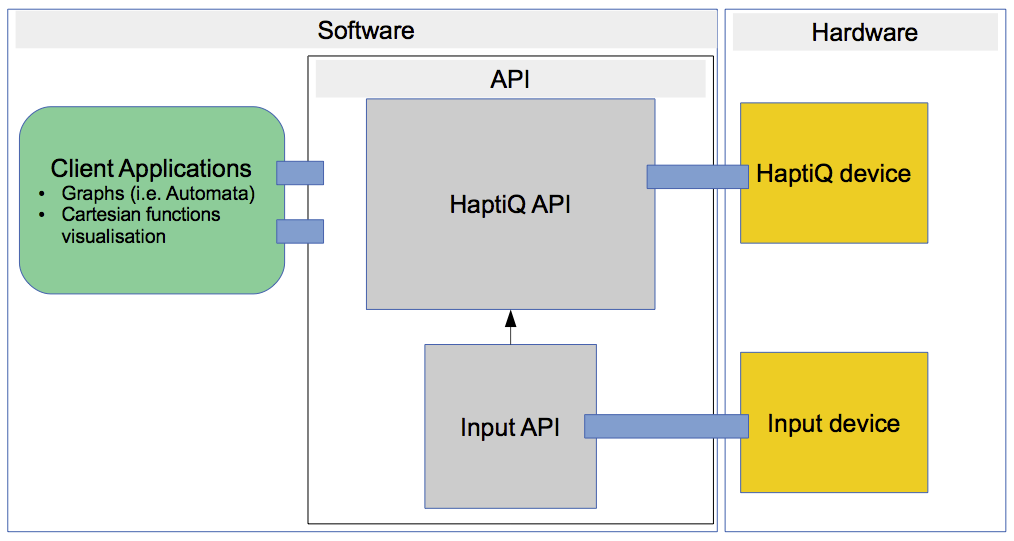
\includegraphics[width=1.0\textwidth]{General_overview.png}
  \caption{API General Overview}
  \label{fig:api}
\end{figure}

\subsection{Input API}

Initially, the HaptiQ, like the HTP, was designed to work on a Microsoft PixelSense table only \cite{pixelsense}.
Microsoft Surface Bytetags are located underneath the HTP to get the location of the device in the table. However, official Bytetags are expensive and printing them with a normal printer does not lead to satisfying results. In addition, the HaptiQ will be used in the near future on digital tables that do not support the Surface SDK. Therefore, in order to abstract the HaptiQ API from any hardware input dependence, a separate API component has been created (see Figure ~\ref{fig:input_api}). 

The architectural structure of the Input API is based on the classic Factory pattern. This adds a level of abstraction over the hardware that should be used to get the position of the HaptiQ. Currently the API supports Bytetags and Glyphs recognition. But client applications can also add their own customised class to support different position detection methods. 

\begin{figure}[H]
  \centering
  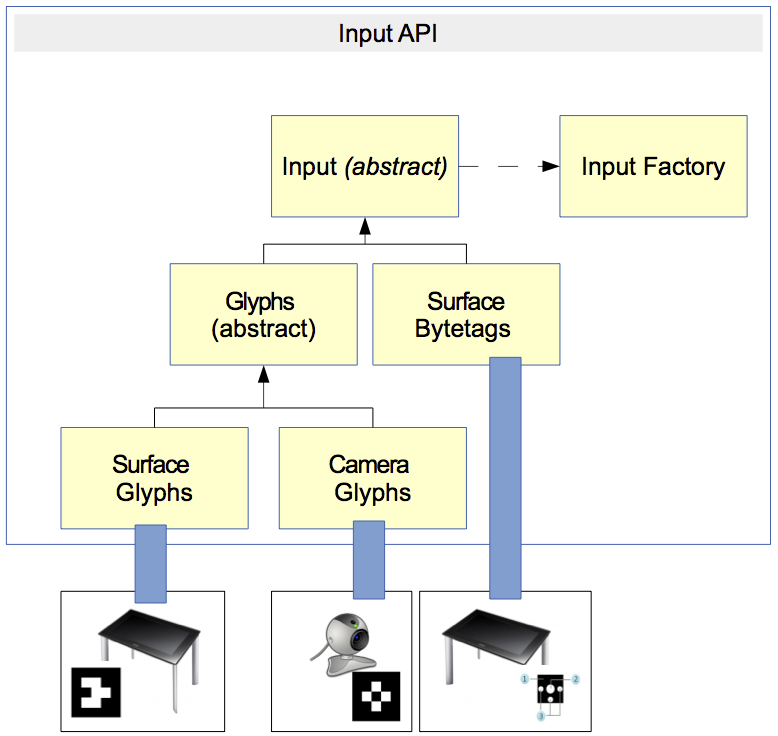
\includegraphics[width=0.5\textwidth]{input.png}
  \caption{Input API}
  \label{fig:input_api}
\end{figure}

\subsection{HaptiQ API}

The HaptiQ API plays the main role within the API by connecting the Input API, the HaptiQ device and the client applications all together (see Figure ~\ref{fig:haptiQ_api}). 

The HaptiQsManager is designed using the Singleton pattern, ensuring that only one instance exists, and controls the different parts of the internal structure of the HaptiQ API. On creation, the manager launches the configuration manager. At this stage, the API looks in the current directory for pre-saved configurations of HaptiQs. If there are not valid configurations matching the current attached devices to the machine, a configuration windows form is started, allowing users to set up devices. Otherwise, HaptiQ objects are created for each configured device. 

Each HaptiQ is a thread process on its own, which runs the current behaviours cyclically. The HaptiQ class is responsible both for controlling the actuators and getting the input via the pressure sensors. 

The manager, however, is responsible to get the devices position through the Input API. Using the observer pattern, the HapticObjects registered by the client applications are notified whenever a new input is received. If the input is relevant to a particular HapticObject, then a behaviour is returned to the HaptiQ device that caused it. 

The API allows behaviours to be added, removed, and substituted. This means that the current state of a device can be the combination of multiple behaviours. This adds an extra dimension to the haptic cues that can be transferred to the user. 

On the other hand, each HaptiQ can keep track of pressure events, without the intervention of the HaptiQsManager. Pressure data events are automatically fired to registered HapticObjects. Each HapticObject reacts differently to pressure input. 

\begin{figure}[H]
  \centering
  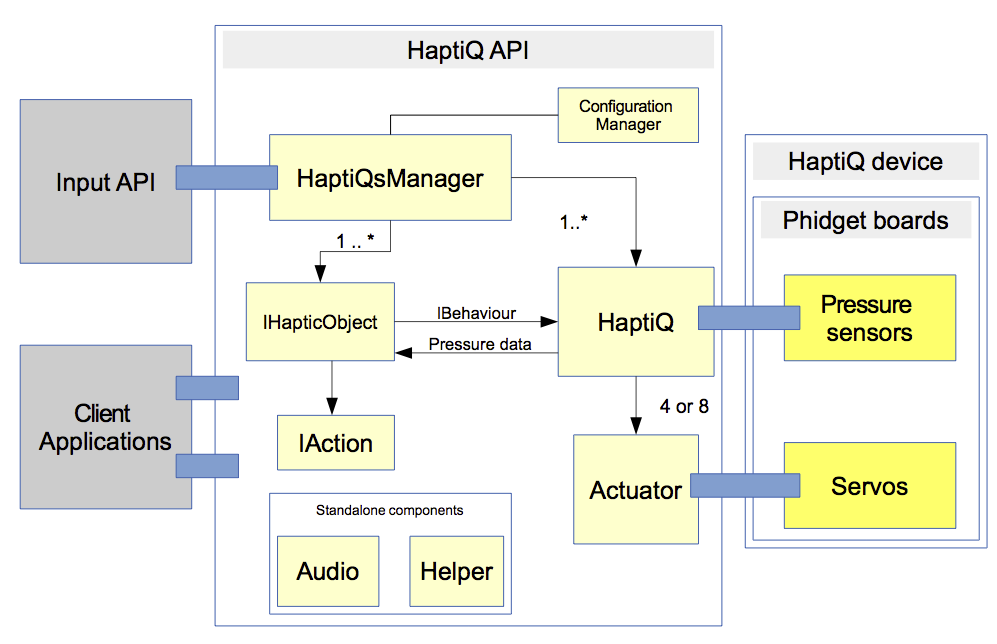
\includegraphics[width=1.0\textwidth]{haptiQAPI.png}
  \caption{HaptiQ API}
  \label{fig:haptiQ_api}
\end{figure}

\subsubsection{Haptic Objects}
Basic haptic objects are provided by the API and are designed to be used by WPF applications without having to concern about behaviours and additional low level mechanisms. All haptic objects can carry textual information. In fact, applications should prioritise the information one wants to convey, rather than the aesthetics of the objects. Therefore, only simple shapes are provided. Obviously, one can extend the HapticShape abstract class to provide more interesting shapes, but this is outside the scope of this project.

Haptic objects are the main visual components of the client applications. Therefore, clients can also register custom actions to be run when pressure events are received by a specific object.

Figure ~\ref{fig:hapticObjects} shows examples of the haptic objects supported by the API. 

The Fiducial Markers used do not provide very precise input location of the device. In order to compensate, the HapticObjects provided are extended (red borders in Figure ~\ref{fig:hapticObjects}). This makes it harder to the user to leave the object, which is wanted behaviour.

\begin{figure}[H]
  \centering
  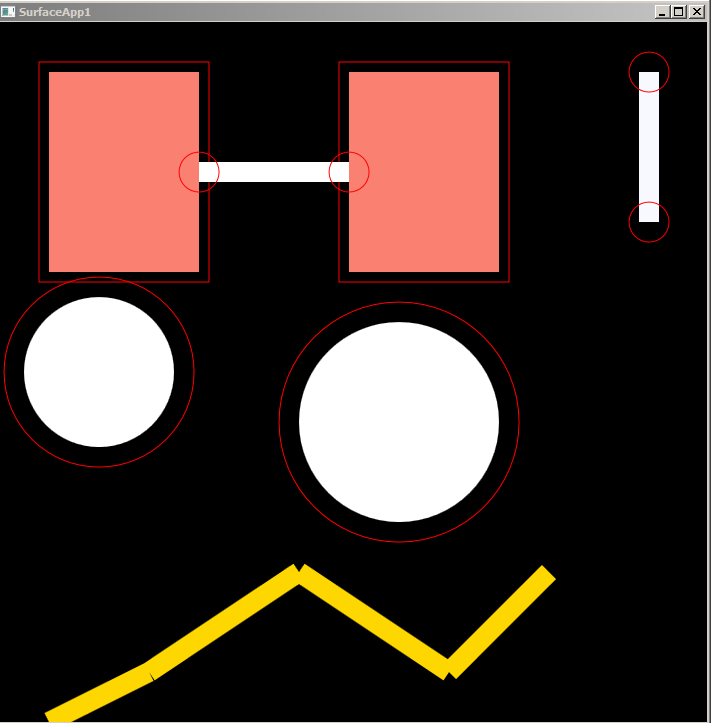
\includegraphics[width=0.7\textwidth]{hapticObjects.png}
  \caption{Haptic Objects. From left-to-right, from top-to-bottom: HapticRectangle (HR), HapticLinks, HR, HapticLine, HapticCircle (HC), HC, HapticPolyline}
  \label{fig:hapticObjects}
\end{figure}

\todo[noline]{add better screenshot}

\subsubsection{Audio Feedback}

The audio component is a standalone one, allowing any part of the API, as well as client applications, to output beeps or textual information as audio.

While this is a small component, it still plays an important role in the API. Ungar and Blades \cite{ungar2000can} discuss whether the conjoint retention hypothesis, combining spatial and linguistic information, can provide richer haptic cueing. Their study did not show any significant improvement when adding audio feedback. However, they results were not definitive. Therefore, I decided to follow the trend of many commercial applications, like VoiceOver, which use audio to provide textual and position feedback too.

In the API provided, the Beep feedback is used only for HapticLines and HapticPolylines. The reason is that following lines is harder than identifying the existence of shapes. This approach is similar to the one taken in audio feedback applications, such as VoiceOver.

The speech synthesiser, instead, is used to read out textual information stored in the HapticObjects.

\section{Tactons}
\label{sec:designTactons} 

Pietrzak et al. \cite{pietrzak2009creating} propose a set of tactons that can be used on pin array devices and that could be used to indicate edges and directions. These tactons are designed for a 4x4 pins grid. The HaptiQ provides a maximum of eight actuators, uses lines rather than points to convey haptic cues and can provide height information as well (pin arrays typically provide only 0/1 information). Here, I present a new set of tactons. In this section the terms tacton and behaviour will be used interchangeably.

A tacton is used by an HapticObject to notify a device how to react when this is located on top of it. In the provided API there is a strong relationship between each HapticObject and a behaviour. Nonetheless, behaviours can be used by client defined HapticObjects or directly from a client application.

In the following sections, the scales in Figure ~\ref{fig:scales} will be used to represent the heights of the actuators.

\begin{figure}[H]
        \centering
        \begin{subfigure}[H]{0.7\textwidth}
                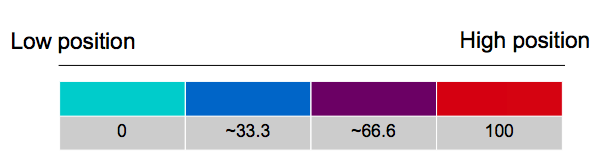
\includegraphics[width=\textwidth]{scaleA.png}
                \caption{4-HaptiQ}
                \label{fig:scale-4}
        \end{subfigure}%
        ~ %add desired spacing between images, e. g. ~, \quad, \qquad etc.
          %(or a blank line to force the subfigure onto a new line)
          
        \begin{subfigure}[H]{0.7\textwidth}
                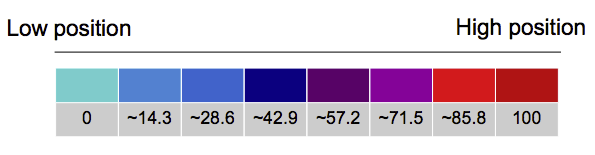
\includegraphics[width=\textwidth]{scaleB.png}
                \caption{8-HaptiQ}
                \label{fig:scale-8}
        \end{subfigure}
        ~ %add desired spacing between images, e. g. ~, \quad, \qquad etc.
        \caption{Blue-Red scale used to indicate the height of the actuators in tactons diagrams. Numerical values represent the positions of the actuators in percentage}
        \label{fig:scales}
\end{figure}

\subsection{Flat and Max}

Flat and Max are the simplest tactons of the set (see Figure ~\ref{fig:Basictactons}). The Flat tacton is typically used to indicate that underneath the device there are no objects or information. The Max behaviour, instead, can be used to represent the existence of an object. For instance, when the device is inside an HapticRectangle the Max behaviour is played. 

\begin{figure}[H]
  \centering
  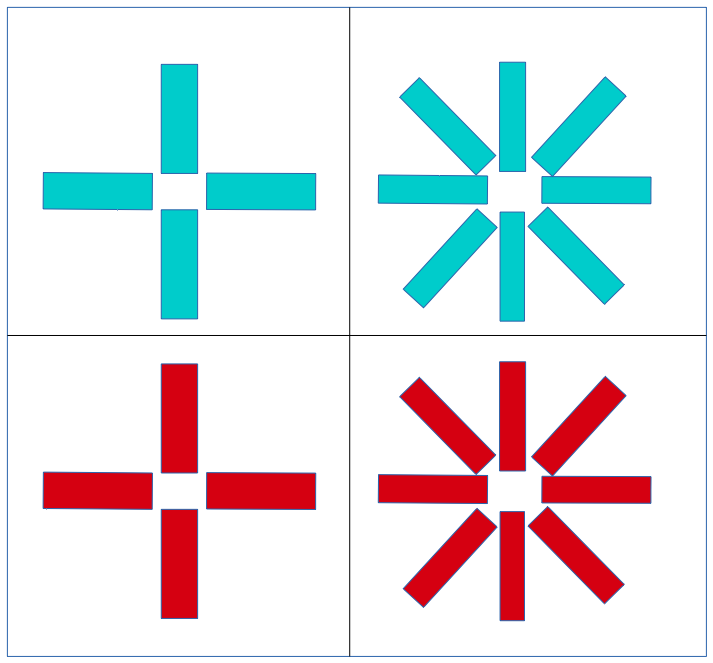
\includegraphics[width=0.5\textwidth]{basic.png}
  \caption{Basic tactons: Flat and Max}
  \label{fig:Basictactons}
\end{figure}

\subsection{Notification}

The Notification tacton, similarly to the Max tacton, can also be used to notify an object. In the case being, this tacton is used to notify an HapticCircle. This tacton consists into cyclically changing the positions of the actuators (see Figure ~\ref{fig:notification}). Each rod always increases or decreases its height position. But in the case the maximum or minimum height threshold is reached, the actuator direction (increase or decrease in height) is inverted.

\begin{figure}[H]
        \centering
        \begin{subfigure}[H]{0.7\textwidth}
                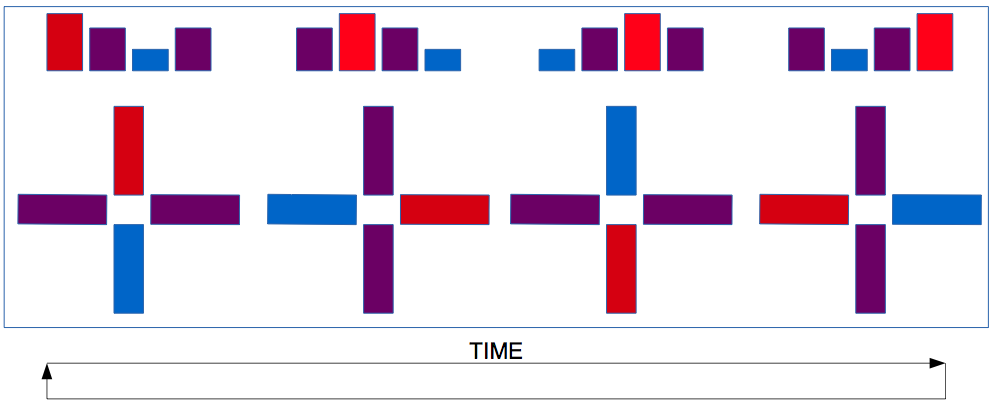
\includegraphics[width=\textwidth]{notification-4.png}
                \caption{4-HaptiQ}
                \label{fig:notification-4}
        \end{subfigure}%
        ~ %add desired spacing between images, e. g. ~, \quad, \qquad etc.
          %(or a blank line to force the subfigure onto a new line)
          
        \begin{subfigure}[H]{0.7\textwidth}
                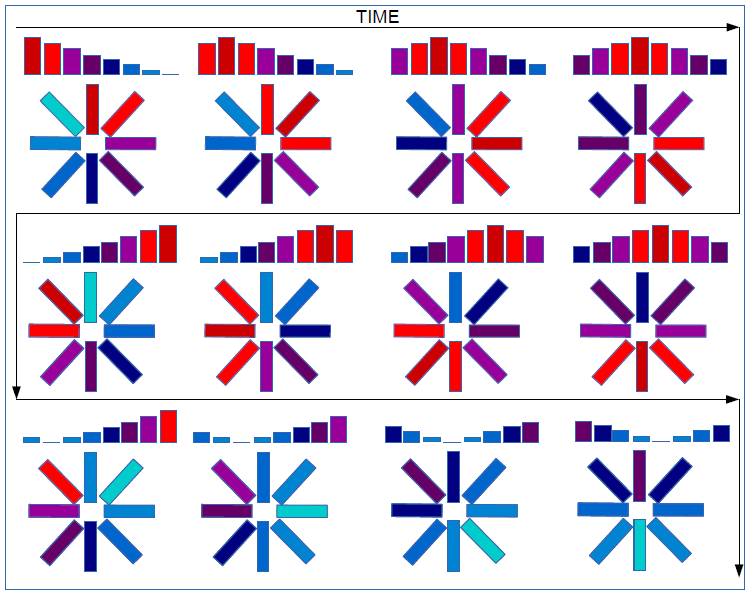
\includegraphics[width=\textwidth]{notification-8.png}
                \caption{First 12 cases for 8-HaptiQ}
                \label{fig:notification-8}
        \end{subfigure}
        ~ %add desired spacing between images, e. g. ~, \quad, \qquad etc.
        \caption{Notification tacton}\label{fig:notification}
\end{figure}

\subsection{Direction}

The Direction tacton \todo[noline]{rename to edge?} is probably the most significant one of all the tactons. This allows the HaptiQ to represent edges and corners. 

Figure ~\ref{fig:edges} show how the combinations of actuators, in both the prototypes, are used to represent edges. The resolution of the device is increased by alternatively actuating adjacent actuators. It is possible to achieve a precision of 45° and 22.5° for the 4-HaptiQ and the 8-HaptiQ respectively. 

\begin{figure}[H]
        \centering
        \begin{subfigure}[H]{0.3\textwidth}
                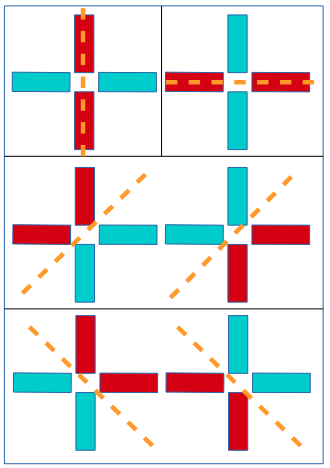
\includegraphics[width=\textwidth]{direction-4.png}
                \caption{4-HaptiQ}
                \label{fig:direction-4}
        \end{subfigure}%
        ~ %add desired spacing between images, e. g. ~, \quad, \qquad etc.
          %(or a blank line to force the subfigure onto a new line)
        \begin{subfigure}[H]{0.5\textwidth}
                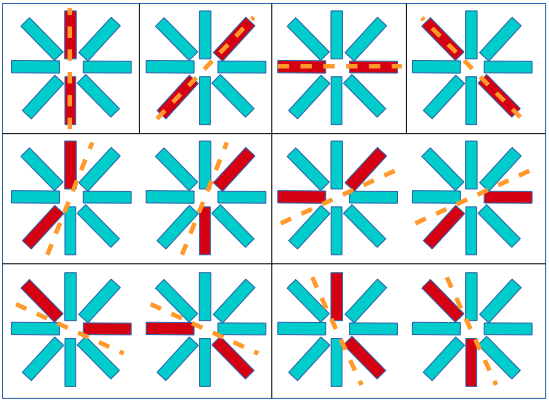
\includegraphics[width=\textwidth]{direction-8.png}
                \caption{8-HaptiQ}
                \label{fig:direction-8}
        \end{subfigure}
        ~ %add desired spacing between images, e. g. ~, \quad, \qquad etc.
        \caption{Direction tacton - Edges}\label{fig:edges}
\end{figure}

It is also possible to represent corners, which are merely the combinations of two edges. The 4-HaptiQ can represent corners of 90° with a precision of 45° (see Figure ~\ref{fig:corner-4}). Indeed, the 8-HaptiQ can represent corners of 45°, 90° and 135°, with a precision of 22.5° (see Figures ~\ref{fig:corner-8}, ~\ref{fig:corner-8c}). 

\begin{figure}[H]
        \centering
        \begin{subfigure}[H]{0.5\textwidth}
                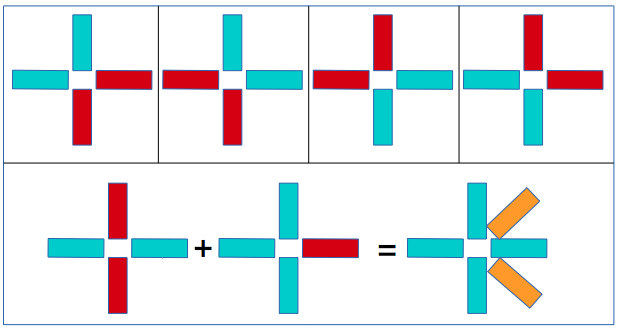
\includegraphics[width=\textwidth]{corners-4.png}
                \caption{4-HaptiQ}
                \label{fig:corner-4}
        \end{subfigure}%
        ~ %add desired spacing between images, e. g. ~, \quad, \qquad etc.
          %(or a blank line to force the subfigure onto a new line)
          
        \begin{subfigure}[H]{0.4\textwidth}
                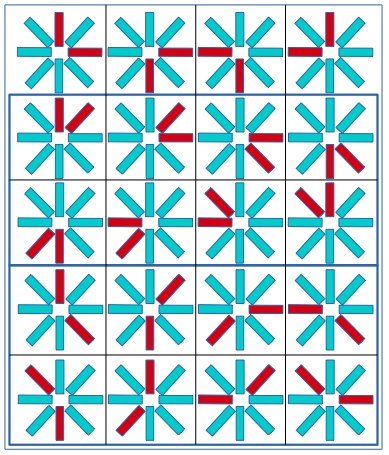
\includegraphics[width=\textwidth]{corners-8.png}
                \caption{8-HaptiQ}
                \label{fig:corner-8}
        \end{subfigure}
        ~ 
         \begin{subfigure}[H]{0.4\textwidth}
                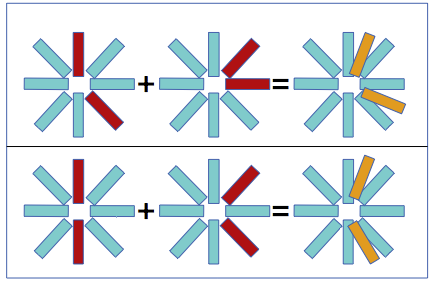
\includegraphics[width=\textwidth]{corners-8c.png}
                \caption{8-HaptiQ (combinations)}
                \label{fig:corner-8c}
        \end{subfigure}
        ~ %add desired spacing between images, e. g. ~, \quad, \qquad etc.
        \caption{Direction tacton - Corners}\label{fig:corners}
\end{figure}

The Direction tacton is used by the HapticRectangle, to represent its borders, and the HapticLine and HapticPolyline objects. 

\subsection{Pulsation and Linear}
The Pulsation and Linear tactons are used with the HapticLink to represent the sign of the link between two Haptic objects. Figure ~\ref{fig:pulsation} shows two cases of the pulsation tacton for the 4-HaptiQ. By symmetry it is possible to represent 8 (or 16 for the 8-HaptiQ) directions. This tacton also allows frequency to be specified, so that pulsation increases as one gets closer to the target. 

The Linear tacton, on the other hand, is the union of the pulsation tactons with not pulsation. One can also specify a linear factor, so that the height of the actuators increases linearly as one gets closer to the target. 

\begin{figure}[H]
  \centering
  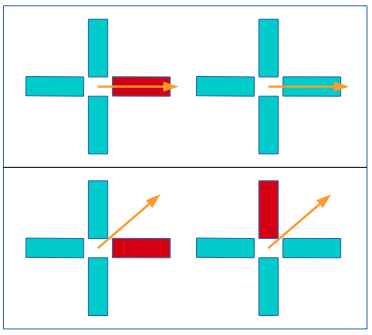
\includegraphics[width=0.5\textwidth]{pulsation.png}
  \caption{Pulsation tacton}
  \label{fig:pulsation}
\end{figure}

\section{Applications}

The HaptiQ can provide a new set of haptic cues which allow the visually impaired to better perceive lines, edges and directions. Two example basic applications have been implemented using the API previously described.

\textbf{Emphasis on the fact that these are just proof-of-concepts, not finished applications}

\subsection{Graphs visualisation}

\subsection{Functions visualisation}

\newpage
\chapter{Implementation}

This content of this chapter follows from the Design chapter.
\newpage
\chapter{Evaluation}

\todo{future work section ?}

\begin{itemize}
	\item feedback from Saad and Regis?
    \item alternative actuators positions (see Piatrzak paper: Creating usable pin array tactons for nonvisual information)
    \item can use hidden-markov-model or time-series-analysis to identify patterns in pressure input and classify gestures
    \item evalute the learning rate for blind people in terms of behaviours of the device
    \item possible experiment --> use of MHTP with audio VS audio only (like VoiceOver in iphone)
\end{itemize}
\newpage
\chapter{Future Work}
\label{chap:futureWork}

The HaptiQ aims to take the Haptic Tabletop Puck to the next level, by allowing the visually impaired to sense edges, corners and directions, and still keeping the hardware inexpensive. In the future, I plan to pursue additional work in collaboration with Régis Ongaro-Carcy, Saad Attieh, and Dr Miguel A. Nacenta. This chapter intends to highlight the potential work that could be planned for the near future, as well as the work currently pursued by Régis Ongaro-Carcy and Dr Miguel A. Nacenta. 

One of the aims of this project is to distribute this work under the GNU General Public License. We believe that the HaptiQ can facilitate blind people to use interactive surfaces without having to spend a considerable amount of money and still providing a sufficient haptic-audio feedback quality. 
The next iteration of the HaptiQ will focus on improving the design and mechanics of the device. The current version is easy to print, but requires about 10 hours of assembling. It is important to redesign some of the pieces and part of the structure of the device, making the HaptiQ more modular and easy to access to people with no experience with 3D printing and models construction. 

In this work no user study was conducted. While the HaptiQ seems to perform very well, it is still unknown how helpful the provided tactons are. A user study with people with visual impairments could help understand how the design, mechanics, and tactons of the HaptiQ perform. Whether a vector-based haptic feedback display provides more helpful cues to the blind and visually impaired when following a line, or on recognising a corner, is unknown. The current device supports modular actuators, so it is possible to compare the vector-based HaptiQ with a grid-based one. A study analysing the current HaptiQ will help to understand how well the current device performs and what is to be improved, added, or removed in the next iteration phase. For instance, it would be very interesting to compare technology similar to VoiceOver \cite{voiceOver}, that uses audio feedback only, with the HaptiQ that uses both haptic and audio feedback (or haptic only). An improved version of the function visualiser application, for instance, would help understanding how well blind people can follow lines using the HaptiQ.  

Future work will consist into exploring what new features should be added to the HaptiQ and its API. New types of haptic objects and behaviours could make the API more powerful, allowing client applications to describe more scenarios. The use of electro-vibration and/or mechanical vibrations could allow the HaptiQ to sense textures. This would be a powerful feature, since the aim of HaptiQ is to compensate for the flat and haptic-less interactive surfaces. Adding a break, like the HTP \cite{marquardt2009haptic} does, would add a new dimension to the HaptiQ: friction. Providing resistance to movements parallel to the used surface can allow applications to represent certain types of textures. There are also other possibilities. For example, different meanings can be given to objects that exert different opposing forces to the movement of the HaptiQ. 

Currently, Régis is developing a strategic game, based on geographical information, for visually impaired people. He is working under the supervision of Dr Miguel A. Nacenta and will conduct a user study with visually impaired people at the Université de Toulouse. While he is working on his research, I will provide support with the HaptiQ, being the main developer. I am also planning to actively participate in the design and development of the game, with the permission of Régis and Dr Nacenta. 
\newpage
\chapter{Conclusions}

Technology, in the last decade, has become always more ubiquitous. However, little effort has been spent on enabling the digital world to be used by people with disabilities. Blind people, in particular, have to face considerable difficulties when trying to access textual and visual information. While, screen readers are able to convey textual information with a good degree of success, the same is not true for more graphical data.

This project presents the HaptiQ, an inexpensive haptic-audio feedback device that the visually impaired can use on interactive surfaces to explore both textual and graphical information. The main focus of the HaptiQ is to facilitate the blind to sense edges, corners and directions. 




\newpage
\bibliographystyle{acm}
\bibliography{bibliography}

\newpage
\begin{appendices}
\chapter{MHTP API}
The contents...
Is this section actually necessary?
\end{appendices}

\end{document}